\documentclass[11pt]{article}
\usepackage[T1]{fontenc}
\usepackage[utf8]{inputenc}
\usepackage{lmodern}
\usepackage[margin=1in]{geometry}
\usepackage{microtype}  % better line breaking + character protrusion

% Global line-break tolerance for long math identifiers
\emergencystretch=2em
\tolerance=1500
\hbadness=10000

% Allow line breaks inside inline math at relation/binary operators
\binoppenalty=700
\relpenalty=500
\usepackage{amsmath,amssymb,amsthm,mathtools,bm,mathrsfs}
\usepackage{longtable,booktabs,array,multirow}
\usepackage{textcomp}
\usepackage{graphicx}
\usepackage{enumitem}
\usepackage{xcolor}
\usepackage{framed}
\usepackage{fancyvrb}
\usepackage{ragged2e}
\usepackage{hyperref}
\usepackage{xurl}
\usepackage{tikz}
\usepackage{tikz-cd}
\usetikzlibrary{arrows.meta, positioning, calc, shapes.geometric, fit, decorations.pathreplacing}
\usepackage{caption}

% Theorem environments
\theoremstyle{plain}
\newtheorem{theorem}{Theorem}[section]
\newtheorem{lemma}[theorem]{Lemma}
\newtheorem{proposition}[theorem]{Proposition}
\newtheorem{corollary}[theorem]{Corollary}

\theoremstyle{definition}
\newtheorem{definition}[theorem]{Definition}
\newtheorem{example}[theorem]{Example}
\newtheorem{remark}[theorem]{Remark}
\newtheorem{convention}[theorem]{Convention}

% Custom commands
\newcommand{\RS}{\mathrm{R\text{-}S}}
\newcommand{\cS}{\mathcal{S}}
\newcommand{\cF}{\mathcal{F}}
\newcommand{\cM}{\mathcal{M}}
\newcommand{\cC}{\mathcal{C}}
\newcommand{\cD}{\mathcal{D}}
\newcommand{\cL}{\mathcal{L}}
\newcommand{\cP}{\mathcal{P}}
\newcommand{\fM}{\mathfrak{M}}
\newcommand{\Meta}{\mathfrak{Meta}}
\newcommand{\LFnd}{\mathcal{L}_{\mathrm{Fnd}}}
\newcommand{\LCls}{\mathcal{L}_{\mathrm{Cls}}}
\newcommand{\LClsMax}{\mathcal{L}_{\mathrm{Cls}}^{\top}}
\newcommand{\LAbs}{\mathcal{L}_{\mathrm{Abs}}}
\newcommand{\Sint}{\cS_{\mathrm{int}}}
\newcommand{\Ob}{\mathrm{Ob}}
\newcommand{\Mor}{\mathrm{Mor}}
\newcommand{\Hom}{\mathrm{Hom}}
\newcommand{\Fun}{\mathrm{Fun}}
\newcommand{\Cl}{\mathrm{Cl}}
\newcommand{\Lan}{\mathrm{Lan}}
\newcommand{\Ran}{\mathrm{Ran}}
\newcommand{\Set}{\mathrm{Set}}
\newcommand{\Cat}{\mathrm{Cat}}
\newcommand{\Syn}{\mathrm{Syn}}
\newcommand{\Mod}{\mathrm{Mod}}
\newcommand{\Con}{\mathrm{Con}}
\newcommand{\PA}{\mathsf{PA}}
\newcommand{\ZFC}{\mathsf{ZFC}}
\newcommand{\MLTT}{\mathsf{MLTT}}
\newcommand{\HoTT}{\mathsf{HoTT}}
\newcommand{\ETT}{\mathsf{ETT}}
\newcommand{\CIC}{\mathsf{CIC}}
\newcommand{\NBG}{\mathsf{NBG}}
\newcommand{\AFA}{\mathsf{AFA}}
\newcommand{\CZF}{\mathsf{CZF}}
\newcommand{\II}{\mathbf{I}}
\newcommand{\cU}{\mathcal{U}}
\newcommand{\tpi}{\widetilde{\pi}}
\newcommand{\cE}{\mathcal{E}}
\newcommand{\fME}{\fM_{\cE}}
\newcommand{\LAbsE}{\LAbs^{\cE}}
\newcommand{\LClsE}{\LCls^{\cE}}
\newcommand{\LClsMaxE}{(\LClsMax)^{\cE}}
\newcommand{\LFndE}{\LFnd^{\cE}}
\newcommand{\SSE}{\cS_{S}^{\cE}}
\newcommand{\SSEbase}{\cS_{S}^{\cE,\,\mathrm{base}}}
\newcommand{\SSEglobal}{\cS_{S}^{\cE,\,\mathrm{global}}}
\newcommand{\Eff}{\ensuremath{\mathsf{Eff}}}
\newcommand{\OWL}{\ensuremath{\mathsf{OWL}}}
\newcommand{\NCG}{\ensuremath{\mathsf{NCG}}}
\DeclareMathOperator{\colim}{colim}
\DeclareMathOperator{\image}{image}
\DeclareMathOperator{\id}{id}
\DeclareMathOperator{\ev}{ev}
\DeclareMathOperator{\Trace}{Trace}
\DeclareMathOperator{\dep}{depth}

\title{The Moduli Space of Formal Systems:\\
Classification, Stabilization, and a No-Go Theorem for Absolute Foundations}

\author{%
  \footnotesize Max Sereda \\[-3pt]
  \scriptsize\textit{Independent researcher} \\[-3pt]
  \scriptsize\texttt{\href{mailto:max@gst.st}{max@gst.st}}%
}

\date{\scriptsize\today}

\begin{document}
\maketitle

\begin{abstract}
I study the $(\infty, n)$-categorical moduli space $\fM$ of formal systems (hereafter \textbf{MSFS}): the classifying $2$-stack of Morita-equivalence classes of Rich-foundations ($\LFnd$ theories satisfying (R1)--(R5)). I establish five structural results and one boundary corollary.

\emph{(i) Plurality at $\LCls$.} The $\infty$-cosmoi (Riehl--Verity), Univalent Foundations (Voevodsky), and cohesive higher topoi (Schreiber) are pairwise non-$2$-equivalent partial meta-frameworks, each classifying a strict sub-stack of $\fM$; they lie outside the rigid maximal sub-class $\Meta_{\mathrm{Cls}}^{\top}$.

\emph{(ii) Conditional meta-categoricity.} Any two members of $\Meta_{\mathrm{Cls}}^{\top}$ over the same Rich-metatheory are $(\infty, \infty)$-equivalent, by Grothendieck--Lurie straightening with joint-faithfulness of the extensional and intensional classification functors.

\emph{(iii) Slice-local intensional refinement.} The display-$2$-class functor $\II : \cF^{\mathrm{op}} \to \Sint$ is slice-local over $\fM$: intensional distinctions ($\MLTT$ vs.\ $\ETT$) fibre over single $\fM$-points, invariantly separated by internal-language computability in Hyland's effective topos $\mathrm{Eff}$.

\emph{(iv) Theory-level meta-stabilization.} Iterated meta-classification reproduces the same $(\infty, \infty)$-theory at each step (Barwick--Schommer-Pries unicity), though set-theoretic instantiation ascends the Grothendieck-universe hierarchy $\kappa_1 < \kappa_2 < \cdots$.

\emph{(v) AC/OC duality.} The Lambek--Scott adjunction $(\Syn, \Mod)$ of (R5b), assembled uniformly across $\RS$ and over $n \in \mathbb{N} \cup \{\infty\}$, induces an $(\infty, \infty)$-equivalence $\fM \simeq \fM_\cE$ between the theory-centric moduli $2$-stack $\fM$ and an enactment-centric moduli $2$-stack $\fM_\cE$ of pointed Rich-enactments. The dual of AFN-T asserts that the enactment-absolute stratum is likewise empty.

\emph{Boundary corollary: the Absolute Foundation No-Go Theorem (AFN-T).} By the syntax--semantics adjunction underlying (R5), $\fM$ has no maximal point: the $\LAbs$ stratum (formally definable, non-reducible, and maximally generative foundation) is empty. AFN-T subsumes the classical no-go series Cantor~\cite{Cantor1891}, Russell~\cite{Russell1903}, G\"odel~\cite{Godel1931}, Tarski~\cite{Tarski1936}, Lawvere~\cite{Lawvere1969}, Ernst~\cite{Ernst2015} uniformly across $\RS$ and all $(\infty, n)$, $n \in \mathbb{N} \cup \{\infty\}$, and extends dually to the enactment-absolute stratum $\LAbs^\cE$.

\smallskip
\noindent\textbf{Keywords:} moduli space of formal systems, classifying $2$-stacks, categorical logic, $(\infty, n)$-categories, higher topos theory, intensional type theory, meta-classification, effective topos, no-go theorems.

\smallskip
\noindent\textbf{MSC2020:} 03A05, 03B30, 03C45, 03F40, 18A05, 18N10, 18N50, 18N60, 18N65.

\end{abstract}

\newpage
\tableofcontents
\newpage

\section{Introduction}

This paper studies the \emph{moduli space of formal systems} $\fM$, the classifying $(\infty, 2)$-stack whose points are Morita-equivalence classes of Rich-foundations (formal theories $F$ satisfying conditions (R1)--(R5) of Definition~\ref{def:rs}) and whose $k$-morphisms are faithful interpretations and provable natural equivalences. The principal results concern the structure of $\fM$:
\begin{itemize}
\item \textbf{Stratification} (\S\ref{sec:hierarchy}): $\LFnd \supsetneq \LCls \supsetneq \LClsMax \supsetneq \LAbs$.
\item \textbf{Structural plurality at $\LCls$} (Theorem~\ref{thm:meta-mult}).
\item \textbf{Conditional categoricity of $\LClsMax$} (Theorem~\ref{thm:meta-cat}).
\item \textbf{Theory-level stabilization with universe-ascent} (Theorem~\ref{thm:meta-stab}).
\item \textbf{Slice-locality of intensional refinement} (Theorem~\ref{thm:slice-locality}).
\item \textbf{Five-axis absoluteness} (\S\ref{sec:five-axis}).
\item \textbf{AC/OC Morita duality} (Theorem~\ref{thm:ac-oc-duality}, Theorem~\ref{thm:dual-afnt}).
\item \textbf{Outer boundary: $\LAbs = \emptyset$} --- the Absolute Foundation No-Go Theorem (Theorem~\ref{thm:afnt-alpha}, Theorem~\ref{thm:afnt-beta}).
\end{itemize}

\subsection{Notation and Conventions}

\begin{convention}\label{conv:zfc-inacc}
I work throughout in $\ZFC$ augmented by two inaccessible cardinals $\kappa_1 < \kappa_2$, providing Grothendieck universes $\mathbf{U}_1 \subset \mathbf{U}_2$ sufficient for the $2$-categorical machinery used. The categorical machinery follows Kelly~\cite{Kelly1982} for enriched and $2$-categories, Lurie~\cite{LurieHTT} for $(\infty, 1)$-categories, Lurie~\cite{LurieHA} for higher algebra, and Riehl--Verity~\cite{RiehlVerity2022} for $\infty$-cosmoi. For accessible functor theory I follow Ad\'amek--Rosick\'y~\cite{AdamekRosicky1994}.
\end{convention}

\begin{convention}[Key symbols]\label{conv:notation}
\begin{itemize}
\item $\cF$ denotes the $2$-category of \emph{Rich-foundations} ($\LFnd$): objects are foundational theories in the sense formalised in \S\ref{sec:rs} below (conditions (R1)--(R5)); $1$-morphisms are faithful interpretations; $2$-morphisms are provable natural equivalences between interpretations.
\item $\rho : \cF \to (\infty, n)\text{-}\Cat$ denotes the \emph{classification functor} assigning to each $F \in \cF$ its category of models (or, for type-theoretic $F$, the syntactic $(\infty, n)$-category $\Syn(F)$).
\item A \emph{gauge transformation} $\tau : F_1 \to F_2$ is a $1$-morphism in $\cF$ accompanied by a distinguished $2$-equivalence $\rho(F_1) \simeq \rho(F_2)$ at the model-categorical level. Two foundations are \emph{gauge-equivalent} if there is an invertible gauge transformation between them. \emph{Relation to Morita equivalence.} Gauge-equivalence at the $\cF$-level corresponds, via the $\fM := \cF/\text{gauge}$ quotient, to Morita equivalence at the stack level: $F_1, F_2 \in \cF$ are gauge-equivalent iff $[F_1] = [F_2]$ in $\fM$, which by construction is the Morita-equivalence class. Throughout the paper, ``gauge'' (1-morphism level) and ``Morita'' (stack level) name the same underlying equivalence relation at their respective categorical strata, related by the $\cF \to \fM$ quotient functor; no distinct third relation is introduced.
\item \emph{Morita-reducibility at the $(\infty, n)$-level}: a $\LAbs$ candidate $X$ and any $Y \in \cS_S$ are each viewed as pointed $(\infty, n)$-categorical structures via the canonical Yoneda embedding into the total $(\infty, n)$-category $\mathbf{StrCat}_{S, n}$ of $S$-structured $(\infty, n)$-categories (Definition~\ref{def:strcat}, stated immediately below). Concretely, $X$ presented by a formula $\phi_X$ corresponds to the pair $(\Syn(S), [\phi_X])$ where $[\phi_X]$ is the isomorphism class of the object defined by $\phi_X$ in the syntactic category; $Y \in \Ob(\cM) \subseteq \cS_S^{\mathrm{local}}$ corresponds to $(\cM, Y)$. I write $X \to_{M, n} Y$, and say $X$ is \emph{Morita-reducible at the $(\infty, n)$-level} to $Y$, if there exists an $(\infty, n)$-functor $\Phi : \Syn(S) \to \cM$ in $\mathbf{StrCat}_{S, n}$ sending $[\phi_X]$ to the isomorphism class of $Y$, with the restriction $\Phi |_{[\phi_X]}$ an $(\infty, n)$-equivalence onto its image. This extends classical ring-Morita equivalence (which compares $\Mod(X)$ and $\Mod(Y)$ as $1$-categories) by incorporating the full $(\infty, n)$-categorical structure; the two notions coincide when $X, Y$ are $1$-categorical and $n = 1$. I use the shorthand ``Morita-equivalent'' for the symmetric notion and ``Morita-reducible'' for the directed version.
\item $\fM$ denotes the \emph{classifying $2$-stack} of $\cF$: the quotient $\fM := \cF / \text{gauge}$, regarded as an $(\infty, 2)$-stack of Morita-equivalence classes of Rich-foundations. Formally, $\fM$ is the straightening of the Cartesian fibration $\int \rho \to \mathrm{R\text{-}S}$ whose fiber over $S$ is the $2$-groupoid $\rho^{-1}(S)$ of foundations over $S$ modulo gauge. The construction follows Lurie HTT~\cite{LurieHTT} \S 3.2 (straightening--unstraightening of Cartesian fibrations).
\item For a $2$-category $\mathbf{F}$, $\mathrm{Aut}_2(\mathbf{F})$ denotes the $2$-group of $2$-autoequivalences $\mathbf{F} \xrightarrow{\simeq_2} \mathbf{F}$ (monoidal under composition, with invertible $1$-morphisms and coherent $2$-cells).
\item $\Sint$ denotes the $2$-category of display $2$-categories (rigorous definition deferred to Appendix~\ref{app:categorical} below).
\item All $2$-categories are locally small and $\kappa_1$-accessible unless stated otherwise. (For specific Rich-foundations $S$ whose consistency strength requires the second inaccessible, the $\Syn(S)$-accessibility parameter generalizes to $\kappa_S \in \{\kappa_1, \kappa_2\}$ per the accessibility clause (R5a) of the Rich-metatheory definition, formalised in \S\ref{sec:rs} below; subsequent $\kappa_1$-statements should be read uniformly as $\kappa_S$-statements where $S$ is indexed by the specific $\LFnd$-point under consideration. All proofs in this paper are stable under this uniform reading, since the accessibility arguments invoke only regularity of the cardinal, not its specific value.)
\item \emph{Truncation and lifting across depths}: for $n \leq n_S$ I write $\Syn^{(\infty, n)}(S) := \tau_{\leq n}(\Syn(S))$ for the $(\infty, n)$-truncation of the syntactic category. For $n > n_S$ I write $\Syn^{(\infty, n)}(S)$ for the canonical $(\infty, n)$-lifting, obtained by left Kan extension of $\Syn(S)$ along the inclusion $(\infty, n_S)\text{-}\Cat \hookrightarrow (\infty, n)\text{-}\Cat$ (Lurie HTT~\cite{LurieHTT} \S 5.4). Under this convention, comparisons between an object $X$ at level $n$ and an $S$-definable object $Y$ at the native depth $n_S$ take place at level $\max(n, n_S)$ via the canonical lifts; when $n = \infty$, the colimit $\colim_{k < \infty} \Syn^{(\infty, k)}(S)$ is the resulting ambient.
\end{itemize}
\end{convention}

\begin{definition}[The total $(\infty, n)$-category $\mathbf{StrCat}_{S, n}$]\label{def:strcat}
For $S \in \RS$ and $n \in \mathbb{N} \cup \{\infty\}$, the \emph{total $(\infty, n)$-category of $S$-structured $(\infty, n)$-categories}, denoted $\mathbf{StrCat}_{S, n}$, has:
\begin{itemize}
\item \textbf{Objects}: pairs $(\cC, \mathrm{str}_\cC)$ where $\cC$ is a $\kappa_1$-accessible $(\infty, n)$-category and $\mathrm{str}_\cC$ is an $S$-model structure on $\cC$ (i.e., an interpretation of $S$-signature into $\cC$ satisfying the axioms of $S$).
\item \textbf{$1$-morphisms}: $S$-preserving $(\infty, n)$-functors $\Phi : (\cC_1, \mathrm{str}_1) \to (\cC_2, \mathrm{str}_2)$, i.e., functors commuting with the respective $S$-model structures up to coherent $(\infty, n)$-isomorphism.
\item \textbf{Higher morphisms}: coherent $(\infty, n)$-natural transformations between $S$-preserving functors.
\end{itemize}
I embed objects of $\Syn(S)$ and of any model $\cM \models S$ into $\mathbf{StrCat}_{S, n}$ via the pointing construction $X \mapsto (\Syn(S), X)$ and $Y \mapsto (\cM, Y)$ respectively. Morita-reducibility, as specified in Convention~\ref{conv:notation}, refers to the existence of an $S$-preserving $(\infty, n)$-functor in $\mathbf{StrCat}_{S, n}$ between such pointed structures that is an equivalence onto its image.
\end{definition}

\section{Stratified Hierarchy of the Moduli Space}\label{sec:hierarchy}

I stratify $\fM$ into four formal strata distinguished by the two structurally distinct meta-operations $\mathrm{Cls}$ (horizontal, classifying) and $\mathrm{Gen}$ (vertical, generative). The strata, defined by their categorical conditions, are:
\[
\LFnd \;\xrightarrow{\mathrm{Cls}}\; \LCls \;\supsetneq\; \LClsMax \;\xrightarrow{\mathrm{Gen}}\; \LAbs.
\]

\begin{figure}[ht]
\centering
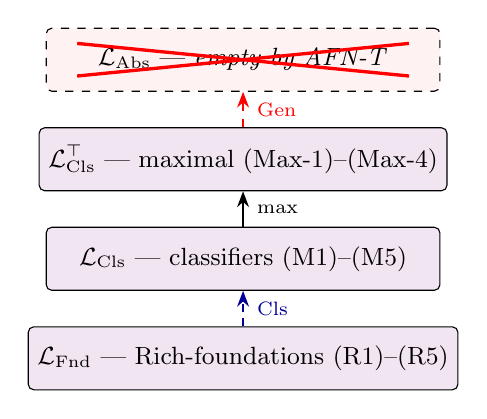
\begin{tikzpicture}[
  level/.style={draw, rounded corners=2pt, minimum width=5cm, minimum height=0.8cm, align=center, font=\small},
  bluefill/.style={fill=blue!6},
  violetfill/.style={fill=violet!10},
  emptybox/.style={draw, dashed, rounded corners=2pt, minimum width=5cm, minimum height=0.8cm, align=center, font=\small, fill=red!5},
  novelty/.style={-{Stealth[length=2mm]}, thick},
  horizmeta/.style={-{Stealth[length=2mm]}, thick, blue!60!black, densely dashed},
  vertmeta/.style={-{Stealth[length=2mm]}, thick, red, dashed},
  node distance=0.45cm
]
\node[level, violetfill] (L5) {$\LFnd$ --- Rich-foundations (R1)--(R5)};
\node[level, violetfill, above=of L5] (L5plus) {$\LCls$ --- classifiers (M1)--(M5)};
\node[level, violetfill, above=of L5plus] (L5max) {$\LClsMax$ --- maximal (Max-1)--(Max-4)};
\node[emptybox, above=of L5max] (L6) {$\LAbs$ --- \emph{empty by AFN-T}};
\draw[horizmeta] (L5.north) -- (L5plus.south) node[midway, right, font=\scriptsize, blue!60!black] {$\,\mathrm{Cls}$};
\draw[novelty] (L5plus.north) -- (L5max.south) node[midway, right, font=\scriptsize] {$\,\mathrm{max}$};
\draw[vertmeta] (L5max.north) -- (L6.south) node[midway, right, font=\scriptsize, red] {$\,\mathrm{Gen}$};
\draw[red, very thick] ($(L6.north west)+(0.4,-0.2)$) -- ($(L6.south east)+(-0.4,0.2)$);
\draw[red, very thick] ($(L6.north east)+(-0.4,-0.2)$) -- ($(L6.south west)+(0.4,0.2)$);
\end{tikzpicture}
\caption{The formal stratification of $\fM$. The blue dashed arrow $\mathrm{Cls}$ denotes the \emph{horizontal meta-operation} (classification without generation; see \S\ref{sec:indexing-scheme}), taking $\LFnd$ to $\LCls$. The maximality restriction selects the sub-class $\LClsMax$. The red dashed arrow $\mathrm{Gen}$ denotes the \emph{vertical meta-operation} (maximal generativity), whose image $\LAbs$ is empty by AFN-T (Theorem~\ref{thm:afnt-alpha}). $\LFnd$ includes $\ZFC$, $\MLTT$, $\HoTT$, $(\infty, 1)$-topos theory, and noncommutative geometry. $\LCls$ partitions into the maximal sub-class $\Meta_{\mathrm{Cls}}^{\top}$ (categorical by Theorem~\ref{thm:meta-cat}) and a plural complement of \emph{partial} classifiers (Theorem~\ref{thm:meta-mult}; $\infty$-cosmoi, Univalent Foundations, cohesive $(\infty, 1)$-topoi), each classifying a strict sub-stack of $\fM$. By Theorem~\ref{thm:ac-oc-duality}, the diagram applies verbatim to the enactment-centric moduli stack $\fM_\cE$ via the $(\infty, \infty)$-equivalence $\fM \simeq \fM_\cE$: the dual strata $\LFndE \to \LClsE \supsetneq \LClsMaxE \to \LAbsE$ mirror the strata above, with $\LAbsE$ likewise empty (Theorem~\ref{thm:dual-afnt}).}
\label{fig:hierarchy}
\end{figure}

\subsection{The Formal Strata}

\begin{definition}[Stratified hierarchy --- formal]\label{def:hierarchy}
I define the formal \emph{strata} as classes of mathematical objects:

\begin{tabular}{@{}ll@{}}
\toprule
Class & Membership criterion \\ \midrule
$\LFnd$ & Formal systems satisfying (R1)--(R5) (specified in \S\ref{sec:rs} below) \\
$\LCls$ & Classifiers satisfying (M1)--(M5) (specified in \S\ref{sec:meta} below) \\
$\LClsMax$ & Classifiers additionally satisfying (Max-1)--(Max-4) (specified in \S\ref{sec:meta} below) \\
$\LAbs$ & Objects satisfying $(F_S) \wedge (\Pi_{4, S, n}) \wedge (\Pi_{3\text{-max}, S, n})$ for some $(S, n)$ (specified in \S\ref{sec:conditions} below) \\
\bottomrule
\end{tabular}
\end{definition}

\begin{proposition}[Structural properties of the hierarchy]\label{prop:level-structure}
\begin{enumerate}
\item[\textbf{(i)}] \emph{Definability.} Each of the four strata is a (possibly proper) class definable in $\ZFC + 2\text{-inacc}$ augmented by the $2$-categorical machinery of Convention~\ref{conv:zfc-inacc}. For $\LFnd$ the conditions are (R1)--(R5) (\S\ref{sec:rs} below); for $\LCls$ they are (M1)--(M5) (\S\ref{sec:meta} below); for $\LClsMax$ they strengthen to (Max-1)--(Max-4) (\S\ref{sec:meta} below); $\LAbs$ is defined by the triple $(F_S) \wedge (\Pi_{4, S, n}) \wedge (\Pi_{3\text{-max}, S, n})$ for some $(S, n)$ (\S\ref{sec:conditions} below; the structural self-contradiction of this triple, recorded in below, yields Theorem~\ref{thm:afnt-alpha}).
\item[\textbf{(ii)}] \emph{Multi-stratum membership.} $\LFnd$ and $\LCls$ are characterized by logically different condition sets (first-order $(R1)$--$(R5)$ on a formal system vs.\ $2$-categorical $(M1)$--$(M5)$ on a $2$-category). A mathematical object carrying both structures satisfies both sets simultaneously: e.g., Univalent Foundations belongs to $\LCls$, with its underlying $\HoTT$ in $\LFnd$. I write $\mathrm{Stratum}(X) \subseteq \{\LFnd, \LCls, \LClsMax, \LAbs\}$ for the set of formal strata containing $X$.
\item[\textbf{(iii)}] \emph{Strict inclusion at the maximal layer.} $\LClsMax \subsetneq \LCls$. Theorem~\ref{thm:meta-cat} asserts that any two members of $\LClsMax$ parametrized by the same Rich-metatheory are $(\infty, \infty)$-equivalent. Theorem~\ref{thm:meta-mult} produces $\geq 3$ pairwise non-$2$-equivalent members of the complement $\LCls \setminus \LClsMax$: the $\infty$-cosmoi of Riehl--Verity, the Univalent Foundations programme, and the cohesive framework of Schreiber.
\item[\textbf{(iv)}] \emph{Emptiness of the absolute stratum.} $\LAbs = \emptyset$ by Theorem~\ref{thm:afnt-alpha}. Consequently $\LFnd \cap \LAbs = \LCls \cap \LAbs = \LClsMax \cap \LAbs = \emptyset$ trivially.
\end{enumerate}
\end{proposition}

\begin{proof}
\textbf{(i)} Each criterion is first-order-expressible; the specified classes are definable.

\textbf{(ii)} The condition sets concern disjoint aspects of an object: axioms with proof calculus vs.\ $2$-categorical structure with classifying functor. An object carrying both structures satisfies both criteria simultaneously.

\textbf{(iii)} Inclusion from the two sets of conditions specified in \S\ref{sec:meta} below: (Max-1)--(Max-4) strengthen (M1)--(M5). Strictness from the structural multiplicity theorem (Theorem~\ref{thm:meta-mult}, proved in \S\ref{sec:meta} below): $\mathbf{F}_{\mathrm{cosmoi}}, \mathbf{F}_{\mathrm{univalent}}, \mathbf{F}_{\mathrm{cohesive}}$ lie in $\LCls \setminus \LClsMax$ since their classification images are strict sub-stacks of $\fM$, violating (Max-1).

\textbf{(iv)} Immediate from Theorem~\ref{thm:afnt-alpha}.
\end{proof}

\subsection{Examples}

\paragraph{Stratum $\LFnd$.} Foundations, with characteristic features:

\begin{longtable}{@{}p{3.8cm}l p{4cm} p{4.6cm}@{}}
\toprule
Foundation & Year & Originator & Characteristic \\ \midrule
Z (Zermelo) & 1908 & Zermelo & No Replacement \\
ZF/ZFC & 1922 & Zermelo, Fraenkel & Classical set theory \\
ZFC + inacc & 1963+ & Grothendieck & With universes \\
NBG & 1925--40 & von Neumann, Bernays, G\"odel & First-class classes \\
MK & 1955 & Morse, Kelley & Impredicative classes \\
KP/KPU & 1965 & Kripke--Platek & Admissible sets \\
ETCS & 1964 & Lawvere & Elementary category of sets \\
ETCC & 1966 & Lawvere & Elementary theory of categories \\
NFU, NF & 1937, 1988 & Quine, Jensen & Stratified comprehension \\
CZF & 1978 & Aczel & Constructive ZF \\
IZF & 1970s & Friedman & Intuitionistic ZF \\
PA & 1889 & Peano & First-order arithmetic \\
$\mathsf{Z}_2$ & 20c & Hilbert--Bernays & Second-order arithmetic \\
MLTT & 1984 & Martin-L\"of & Dependent types \\
CIC & 1988 & Coquand--Huet & Inductive constructions \\
HoTT & 2005+ & Awodey, Voevodsky & Univalence + identity types \\
Cubical HoTT & 2015+ & Cohen--Coquand et al. & Computational univalence \\
Universe-poly.\ HoTT & 2013+ & Voevodsky & Universe polymorphism \\
Linear logic + ! & 1987 & Girard & Resource-sensitive \\
NBG + AFA & 1988 & Aczel & Non-well-founded sets \\
$(\infty, 1)$-topos theory & 2009 & Lurie & $(\infty, 1)$-topoi \\
Non-commutative geom.\ & 1980s & Connes & Spectral triples \\
Cohesive $(\infty, 1)$-topos & 2013 & Schreiber & Cohesion modalities \\
Motivic $\mathrm{SH}(k)$ & 1999 & Voevodsky, Morel & Motivic homotopy \\
Realizability (Eff) & 1982 & Hyland & Effective topos \\
Markov constructive math & 1950s--1980s & A.A.~Markov, Nagornyj & Constructive analysis + Markov's principle \\
Bishop constructive analysis & 1967 & Bishop, Bridges & Choice-free constructive real analysis \\
Synthetic diff.~geom.\ & 1970s & Kock, Lawvere & Infinitesimals as axioms \\
Elementary higher topos & 2021 & Rasekh & Elementary $(\infty, 1)$-topos \\
\bottomrule
\end{longtable}

\paragraph{Stratum $\LCls$.} Classifiers (meta-frameworks). $\LCls$ partitions into the maximal sub-class $\Meta_{\mathrm{Cls}}^{\top}$ (categorical up to $(\infty, \infty)$-equivalence by Theorem~\ref{thm:meta-cat}) and its complement of \emph{partial} (non-maximal) classifiers, which classify strict sub-stacks of $\fM$ rather than all of $\fM$. The classifiers listed below are all non-maximal: each satisfies (M1)--(M5) but violates (Max-1), as witnessed by the strict-subset character of its classification focus.

\begin{longtable}{@{}p{3.3cm}l p{3cm} p{4.4cm}c@{}}
\toprule
Meta-framework & Year & Originator & Classification focus & In $\Meta_{\mathrm{Cls}}^{\top}$? \\ \midrule
$\infty$-cosmoi & 2022 & Riehl--Verity & $(\infty, 1)$-categorical theories & No \\
Univalent Foundations & 2010+ & Voevodsky & HoTT extensions & No \\
Cohesive framework & 2013 & Schreiber & Cohesive $\infty$-topoi & No \\
Higher Algebra prog.\ & 2017+ & Lurie & Stable $\infty$-cat + operadic & No \\
Synthetic mathematics & 2000s+ & Taylor, Shulman & Axiomatic synthetic foundations & No \\
\bottomrule
\end{longtable}

\paragraph{Stratum $\LAbs$.} Empty, by AFN-T.

\subsection{The Two Meta-Operations}\label{sec:indexing-scheme}

\paragraph{Horizontal and vertical meta.} Two categorically distinct meta-operations act on a stratum $\mathcal{L}$:
\begin{itemize}
\item \textbf{Horizontal (classifying) meta.} $\mathrm{Cls}(\mathcal{L})$ is the class of $2$-categories $\mathbf{F}$ \emph{classifying} but not \emph{generating} members of $\mathcal{L}$: locally small, equipped with an accessible classification functor into the moduli of $\mathcal{L}$, non-generative, and metatheory-parametrized (cf.\ (M1)--(M5)).
\item \textbf{Vertical (generative) meta.} $\mathrm{Gen}(\mathcal{L})$ is the class of frameworks \emph{generating} members of $\mathcal{L}$ as internal derivations --- candidate absolute foundations.
\end{itemize}

\begin{proposition}[Non-collapse of the horizontal meta at $\LFnd$]\label{prop:no-collapse}
$\mathrm{Cls}(\LFnd)$ does \emph{not} embed into $\LFnd$ and does not coincide with $\LAbs$. It is therefore a distinct formal stratum, which I label $\LCls$.
\end{proposition}

\begin{proof}[Proof sketch.]
A member $\mathbf{F} \in \mathrm{Cls}(\LFnd)$ is a $2$-category of Rich-foundations with an accessible classification functor into $\fM$. It is not itself a Rich-foundation (it does not satisfy (R1)--(R5) for a generating theory), so $\mathbf{F} \notin \LFnd$. It is not in $\LAbs$ because (M4) requires non-generativity, while $\LAbs$ requires maximal generativity $(\Pi_{3\text{-max}})$.
\end{proof}

\paragraph{Horizontal stabilization.} Theorem~\ref{thm:meta-stab} asserts that iterating $\mathrm{Cls}$ at $\LCls$ stabilizes \emph{at the theory level}: the twice-iterated moduli realizes the same $(\infty, \infty)$-theory as the once-iterated one (written $\simeq_2$, with the universe-ascent caveat of Theorem~\ref{thm:meta-stab}(b)), so $\mathrm{Cls}(\LCls) \simeq_2 \LCls$. No further horizontal stratum distinct from $\LCls$ arises.

\paragraph{Vertical step to the forbidden stratum.} $\LAbs \supseteq \mathrm{Gen}(\LFnd)$: a member of $\LAbs$ would be a maximally-generative foundation from which all of $\LFnd$ derives. This is categorically a fresh operation, not an iteration of $\mathrm{Cls}$. By AFN-T, $\LAbs = \emptyset$.

\paragraph{Summary.} The formal sequence reads:
\[
\underbrace{\LFnd}_{\text{(R1)--(R5)}} \; \xrightarrow{\mathrm{Cls}} \; \underbrace{\LCls}_{\text{(M1)--(M5)}} \; \supsetneq \; \underbrace{\LClsMax}_{(\mathrm{Max}\text{-1})\text{--}(\mathrm{Max}\text{-4})} \; \xrightarrow{\mathrm{Gen}} \; \underbrace{\LAbs = \emptyset}_{\text{AFN-T}}
\]

\section{Reasonable Rich-Metatheories}\label{sec:rs}

\subsection{Rich-Metatheory Conditions}

\begin{definition}[Reasonable Rich-Metatheory]\label{def:rs}
A theory $S$ formulated in a first-order meta-syntax is a \textbf{reasonable Rich-metatheory} (or \textbf{R-S}) if it satisfies:
\begin{itemize}
\item \textbf{(R1) Arithmetic completeness}: $S$ interprets Robinson arithmetic $\mathsf{Q}$.
\item \textbf{(R2) Recursive enumerability}: the set of axioms of $S$ is recursively enumerable.
\item \textbf{(R3) Model existence}: $S$ has at least one model $\cM$ in the ambient set-theoretic meta-universe $\mathbf{U}_2$ (the outer Grothendieck universe of Convention~\ref{conv:zfc-inacc}, large enough to accommodate models of all listed R-S examples including $\ZFC$ + inaccessible cardinals, whose smallest models have size $\kappa_1$ and therefore lie in $\mathbf{U}_2 \setminus \mathbf{U}_1$).
\item \textbf{(R4) G\"odel coding}: there exists a recursive injection $\ulcorner \cdot \urcorner : \mathrm{Formulas}(S) \to \mathbb{N}$ for which the predicates ``$n$ is the G\"odel number of a provable formula'' and ``$n$ is the G\"odel number of a well-formed formula'' are $S$-definable.
\item \textbf{(R5) Categorical semantics}: there exists $n_S \in \mathbb{N} \cup \{\infty\}$, the \emph{intrinsic categorical depth} of $S$, such that
\begin{itemize}
\item[\textbf{(R5a)}] the syntactic category $\Syn(S)$ of $S$ (objects: contexts; $1$-morphisms: provable-from-context substitutions; higher morphisms: proofs of equality of substitutions) is a $\kappa_S$-accessible $(\infty, n_S)$-category, where $\kappa_S \in \{\kappa_1, \kappa_2\}$ is determined by $S$: for $S$ of consistency strength $\leq \kappa_1$ (e.g., $\ZFC$, $\PA$, $\HoTT$, $\MLTT$, $\CIC$) set $\kappa_S = \kappa_1$; for $S$ of consistency strength requiring the second inaccessible (e.g., $\ZFC$ + inaccessible) set $\kappa_S = \kappa_2$. The accessibility parameter follows the theory's consistency strength; all theorems below are stated uniformly for arbitrary $\kappa_S \in \{\kappa_1, \kappa_2\}$ unless a specific case is flagged;
\item[\textbf{(R5b)}] the syntax-to-semantics evaluation $\ev : \Syn(S) \to \cM$ for every model $\cM \models S$ is an $S$-preserving $(\infty, n_S)$-functor, and the pair of functors $(\Syn, \Mod)$ constitutes a Lambek--Scott-type adjunction whose unit at $\Syn(S)$ is an $(\infty, n_S)$-equivalence onto the \emph{initial $S$-structured $(\infty, n_S)$-category}, i.e., the initial object in the $(\infty, n_S + 1)$-category of $S$-structured $(\infty, n_S)$-categories and $S$-preserving $(\infty, n_S)$-functors between them.
\end{itemize}
The Lambek--Scott adjunction of (R5a)--(R5b) at level $n_S$ is established by the composition: Lambek--Scott~\cite{LambekScott1986} for $n_S = 1$; Kapulkin--Lumsdaine~\cite{KapulkinLumsdaine2021} and Awodey--Warren~\cite{AwodeyWarren2009} for $n_S = \infty$ in the HoTT sense; Barwick--Schommer-Pries~\cite{BarwickSchommerPries2021} unicity together with Bergner--Rezk~\cite{BergnerRezk2013} model comparison and Gagna--Harpaz--Lanari~\cite{GagnaHarpazLanari2021} $(\infty, 2)$-straightening for general $n_S \geq 2$. Only the structural consequences---$2$-functoriality of $\Syn$, uniqueness of the initial $S$-structured object up to canonical $(\infty, n_S)$-equivalence---are invoked below.
\emph{Note on the intrinsic categorical depth $n_S$.} The parameter $n_S$ denotes the highest $k$ at which $\Syn(S)$ supports structurally non-trivial $k$-morphisms before all higher cells become invertible. For first-order $S$, $n_S = 1$. For Martin-L\"of type theory and HoTT with univalence, the syntactic category is \emph{an} $(\infty, 1)$-category in the standard terminology (Kapulkin--Lumsdaine~\cite{KapulkinLumsdaine2021}); the notation $n_S = \infty$ in this paper refers to the \emph{unbounded iteration of identity-type formation} producing non-trivial higher-equality content at every finite level $k \in \mathbb{N}$, i.e., no $k$ at which all structure becomes $(k-1)$-truncated. This ``unbounded depth'' reading is an iterative notion and is \emph{not} the same as the $(\infty, \infty)$-categorical notion of Rezk / Barwick--Schommer-Pries~\cite{BarwickSchommerPries2021} (where $k$-morphisms at every $k$ are \emph{non-invertible}). Both readings agree on the behaviour of AFN-T (Theorem~\ref{thm:vertical}), and no argument in the paper depends on the distinction.

Instances verifying (R5a)--(R5b): first-order $S$ at $n_S = 1$ (Lambek--Scott~\cite{LambekScott1986}); Martin-L\"of type theory with $n_S = \infty$ (Awodey--Warren~\cite{AwodeyWarren2009}); HoTT with $n_S = \infty$ (Kapulkin--Lumsdaine~\cite{KapulkinLumsdaine2021}); dependent type theories (Jacobs~\cite{Jacobs1999}).
\end{itemize}
\end{definition}

\subsection{Examples of R-S}

The following are reasonable Rich-metatheories. Each entry is a \emph{formal theory} $S$ (axiomatic system with r.e.\ axiomatisation (R2) and interpreting Q (R1)); categorical structures such as topoi appear as \emph{models} of these theories rather than as theories themselves, and are cited through their internal languages.
\begin{itemize}
\item $\ZFC$; $\ZFC$ + inaccessible cardinals; $\NBG$; Morse--Kelley; $\NBG + \AFA$ (Aczel).
\item The intuitionistic type theories $\MLTT$ and $\CIC$; $\HoTT$ with univalence; universe-polymorphic $\HoTT$.
\item \emph{Linear logic with exponential} $!$, equipped with arithmetic constants sufficient to interpret Q (i.e., intuitionistic linear arithmetic, $\mathsf{ILL}_{\mathsf{PA}}$, or the bounded linear arithmetic fragment of Girard's ludics framework~\cite{Girard2001}); purely propositional linear logic does \emph{not} satisfy (R1) and is excluded.
\item The \emph{internal dependent type theory of Lurie's $\infty$-topoi} (the axiomatic presentation of an $(\infty, 1)$-topos as a model of homotopy type theory with univalent universes and higher modalities, Lurie HTT~\cite{LurieHTT} \S 5--\S 6 via the internal-language correspondence of Shulman~\cite{Shulman2019}, Awodey--Warren~\cite{AwodeyWarren2009}); the $(\infty, 1)$-topos itself is a \emph{canonical model} of this theory, not a separate theory.
\item The \emph{internal language of the Cohesive $\infty$-topos} (Schreiber~\cite{Schreiber2013}): $\HoTT$ extended by adjoint triples of modal operators $(\Pi \dashv \flat \dashv \sharp)$ corresponding to the cohesion axioms, formulated as a type-theoretic extension.
\item \emph{Motivic-extended foundations}: $\ZFC$ (or $\HoTT$) extended with axioms asserting the existence of the motivic stable $\infty$-category $\mathrm{SH}(k)$ and its A$^1$-homotopy invariance as a formal Rich-extension; the motivic $\infty$-category itself is again a model-theoretic construct, not a standalone theory.
\item The \emph{internal language of the realizability topos} $\mathrm{Eff}$: intuitionistic higher-order arithmetic with realizability (Hyland~\cite{Hyland1982}), of which $\mathrm{Eff}$ is the canonical model; we use the shorthand ``$\mathrm{Eff}$-theory'' below for this internal language.
\item \emph{Markov constructive mathematics} (Markov, Nagornyj~\cite{MarkovNagornyj1988}: $\mathsf{HA}$ + Markov's principle, with categorical semantics in $\mathrm{Eff}$).
\item \emph{Bishop constructive analysis}~\cite{Bishop1967,BridgesVita2006} (choice-free constructive real analysis with full categorical semantics in any topos with natural number object).
\item \emph{Feferman predicative analysis}~\cite{Feferman1964} ($\mathsf{ATR}_0$-strength systems with predicative comprehension).
\end{itemize}

\subsection{Non-examples}

\begin{itemize}
\item \emph{Affine logic without exponential $!$}: fails (R1) --- Peano induction requires contraction on the induction hypothesis.
\item \emph{Inconsistent theories}: fail (R3).
\item \emph{Second-order arithmetic with full semantics}: fails (R2) --- the full set of valid formulas is not recursively enumerable.
\item \emph{Intuitive ``theories of everything''} in physics lacking formal axiomatization: fail (R1) and (R2).
\item \emph{Strict philosophical ultrafinitism} (Esenin-Volpin~\cite{EseninVolpin1961,EseninVolpin1970}): fails (R1) at the strictest reading --- the totality of the successor function is rejected for ``infeasibly large'' arguments, so full Peano induction is not available. Bounded variants (see Boundary cases below) belong to a different stratum.
\end{itemize}

\begin{proposition}[Independence of (R1)--(R5)]\label{prop:rs-independence}
The five conditions (R1)--(R5) defining the class $\RS$ are pairwise independent: for each $i \in \{1, 2, 3, 4, 5\}$ there exists a theory $T_i$ satisfying all conditions except (R$i$).
\end{proposition}

\begin{proof}[Witnesses]
\begin{itemize}[nosep]
\item \emph{(R1)-failure with (R2)--(R5) holding}: \emph{affine logic without exponential $!$} satisfies r.e.-axiomatizability (R2), has consistent models in $\mathbf{U}_1$ (R3), admits G\"odel coding over its formula set (R4), and possesses a standard categorical semantics in symmetric-monoidal categories (R5 at $n_S = 1$); the failure is (R1): without contraction, full Peano induction on the induction hypothesis is unavailable, so Robinson's Q cannot be interpreted in the standard sense.
\item \emph{(R2)-failure with (R1), (R3)--(R5) holding}: \emph{second-order arithmetic with full (Henkin-external) semantics}. It interprets Q trivially (R1), has full-semantic models (R3), admits G\"odel coding (R4), and has a categorical semantics in $2$-categories (R5). But (R2) fails: the set of theorems valid under full semantics is not r.e.\ (a consequence of second-order incompleteness).
\item \emph{(R3)-failure with (R1), (R2), (R4), (R5) holding}: \emph{$\ZFC + \text{proper class of inaccessibles}$}. It interprets Q (R1), is r.e.-axiomatized (R2), admits G\"odel coding (R4), and its syntactic category is a $\kappa_1$-accessible $(\infty, 1)$-category with the standard Lambek--Scott adjunction (R5). But (R3) fails in the ambient meta-universe $\ZFC + 2\text{-inacc}$: models of this theory require proper-class-many inaccessibles, which cannot be accommodated within $\mathbf{U}_2 = V_{\kappa_2}$ (which contains only two inaccessibles, $\kappa_1 < \kappa_2$). A consistent theory whose consistency-strength exceeds the meta-universe's capacity is the canonical (R3)-failure mode; inconsistent theories, by contrast, also fail (R5b) vacuously and therefore do not cleanly isolate (R3).
\item \emph{(R4)-failure with (R1)--(R3), (R5) holding}: an artificial theory $T$ extending Q in a language whose G\"odel numbering is uncomputable (e.g., using a non-recursive bijection between formulas and natural numbers). (R1)--(R3) and (R5) hold after replaying the Q-interpretation; (R4) fails because the bijection is non-recursive.
\item \emph{(R5)-failure with (R1)--(R4) holding}: \emph{pure first-order Peano arithmetic $\mathsf{PA}$ equipped with a non-standard comprehension schema} that renders the syntactic category non-accessible (e.g., by enlarging the context objects to a proper class via $\mathbf{U}_2$-sized quantifier domains without corresponding $(\infty, n)$-functorial semantics). (R1)--(R4) are inherited from $\mathsf{PA}$; (R5a) fails because $\Syn(T)$ is no longer $\kappa_1$-accessible. More canonically, any theory whose formal language permits comprehension outside the natural number stratum but fails to admit a Lambek--Scott adjunction to a model category constitutes a witness.
\end{itemize}
\end{proof}

\begin{itemize}
\item \emph{Bounded arithmetic and feasibility calculi.} The systems $\mathsf{I\Delta_0}$, $\mathsf{S}_2^i$ / $\mathsf{T}_2^i$ of Buss~\cite{Buss1986}, $\mathsf{V}_0$, polynomial-time computable arithmetics, and proof-theoretic feasibility calculi formalise restricted fragments of the ultrafinitist intuition. They satisfy (R2)--(R5) but realise (R1) only in a restricted form: the ambient arithmetic interprets a bounded-quantifier fragment of $\mathsf{PA}$, not full $\mathsf{PA}$. They are admissible into $\RS$ as \emph{weak Rich-metatheories}, classifying a corresponding sub-stack of $\fM$ at restricted intrinsic categorical depth $n_S$. Their Morita-relation to standard $\RS$-points is studied via reverse mathematics~\cite{Simpson2009}.
\item \emph{Strict ultrafinitism (Esenin-Volpin tradition).} The strictest philosophical ultrafinitism, which rejects the totality of successor for ``infeasibly large'' arguments, falls outside $\RS$ at any standard reading of (R1) (above, Non-examples). The bounded-arithmetic and polynomial-time variants above provide formal reconstructions admissible into $\RS$ as weak Rich-metatheories.
\item \emph{Paraconsistent theories.} Treated separately in Appendix~\ref{app:paraconsistent}: an additional \emph{classical-kernel} construction admits paraconsistent $S$ into $\RS$ via Routley--Meyer semantics, with AFN-T re-derived in this extended setting.
\end{itemize}

\subsection{\texorpdfstring{The Class $\cS_S$}{The Class S\_S}}

\begin{definition}[$S$-definable categorical structures]\label{def:SS}
Let $S \in \RS$. Define inductively:
\begin{align*}
\cS_S^{\mathrm{local}} &:= \{(\cM, Y) : \cM \models S,\ Y \in \Ob(\cM)\} \;\cup\; \{(\Syn(S), X) : X \in \Ob(\Syn(S))\}, \\
\cS_S^{(0)} &:= \cS_S^{\mathrm{local}}, \\
\cS_S^{(k+1)} &:= \cS_S^{(k)} \,\cup\, \mathcal{O}\bigl(\cS_S^{(k)}\bigr),
\end{align*}
where $\mathcal{O}$ is the closure under the following fixed list of $(\infty, n)$-categorical operations, each taking $\cS_S^{(k)}$-objects as input and producing objects in $\cS_S^{(k+1)}$:
\begin{enumerate}[nosep,label=\textrm{(O\arabic*)}]
\item Left and right Kan extensions along $\cS_S^{(k)}$-morphisms;
\item Grothendieck constructions $\int F$ for Cartesian fibrations $F : I \to \cS_S^{(k)}$ with $I \in \cS_S^{(k)}$;
\item Limits and colimits of $\cS_S^{(k)}$-small diagrams;
\item Slice/comma/opposite categories built from $\cS_S^{(k)}$-data;
\item Derived functors (Quillen sense) between $\cS_S^{(k)}$-objects equipped with model-category structure (when applicable; vacuous on objects without model structure);
\item Symmetric monoidal tensor products and internal hom in closed monoidal $\cS_S^{(k)}$-objects.
\end{enumerate}
Set $\cS_S^{\mathrm{global}} := \bigcup_{k < \omega} \cS_S^{(k)}$ and $\cS_S := \cS_S^{\mathrm{local}} \cup \cS_S^{\mathrm{global}}$. All operations (O1)--(O6) are $\kappa_1$-accessible (Ad\'amek--Rosick\'y~\cite{AdamekRosicky1994}); $\cS_S^{\mathrm{global}}$ is $\kappa_1$-accessible and $\mathbf{U}_2$-small.
\end{definition}

\subsection{\texorpdfstring{Key Lemma: $S$-Definability Implies $\cS_S$-Membership}{Key Lemma: S-Definability Implies S\_S-Membership}}

\begin{lemma}[$S$-definability lemma]\label{lem:SS-membership}
If $X$ is a formally $S$-definable object --- meaning $X$ is specified by a formula $\phi_X \in S$ expressing its characteristic properties --- then $X \in \cS_S$.
\end{lemma}

\begin{proof}
$\phi_X$ presents $X \in \Ob(\Syn(F))$ for some $F \subseteq S$, $F \in \cF$. By (R2), (R5a), $\Syn(F)$ is the Grothendieck construction over $\Mod(F)$ (Lurie~\cite{LurieHTT} \S 5.1), a derived functor from $\cS_S^{\mathrm{local}}$-data, so $\Syn(F) \in \cS_S^{\mathrm{global}}$; hence $X \in \cS_S^{\mathrm{global}} \subseteq \cS_S$.
\end{proof}

\subsection{Size Stratification}\label{sec:size-stratification}

\paragraph{Size classes within $\cS_S$.}
\begin{itemize}
\item \textbf{Small} (elements of $\mathbf{U}_1$): sets of rank $< \kappa_1$.
\item \textbf{Large} (elements of $\mathbf{U}_2 \setminus \mathbf{U}_1$): sets of rank in $[\kappa_1, \kappa_2)$.
\item \textbf{Beyond $\mathbf{U}_2$}: sets of rank $\geq \kappa_2$, including $\mathbf{U}_2$-proper classes.
\end{itemize}

\paragraph{Cardinality bounds for ambient structures.}
\begin{itemize}
\item The $S$-definability class $\cS_S = \cS_S^{\mathrm{local}} \cup \cS_S^{\mathrm{global}}$ is $\mathbf{U}_2$-indexed: $\cS_S^{\mathrm{local}} \subseteq \mathbf{U}_1$ (objects of $\mathbf{U}_1$-sized models) and $\cS_S^{\mathrm{global}} \subseteq \mathbf{U}_2$ (derived constructions over $\cS_S^{\mathrm{local}}$ through $\mathbf{U}_2$-bounded functorial operations).
\item $|\Ob(\cF)/\!\simeq| \leq 2^{\aleph_0} < \kappa_1$; $|\cF| \leq \kappa_2$.
\item $|\Ob(\mathbf{StrCat}_{S, n})/\!\simeq| \leq 2^{\kappa_1} < \kappa_2$.
\item $|\fM / \!\simeq_2| \leq \kappa_2$; $\fM^{(\mathrm{Cls}\cdot k)}$ at $\kappa_k$ (Theorem~\ref{thm:meta-stab}(b)).
\end{itemize}

\section{\texorpdfstring{The $\LAbs$ Conditions}{The L\_Abs Conditions}}\label{sec:conditions}

\begin{definition}[$(F_S)$]\label{def:F}
An $(\infty, n)$-category $X$ satisfies $(F_S)$ for $S \in \RS$ iff $\exists F \in \cF$ with:
\begin{itemize}
\item[\textbf{(F-1)}] $\iota_F : F \hookrightarrow S$ (subtheory inclusion);
\item[\textbf{(F-2)}] $\iota_F^* : \Mod(S) \to \Mod(F)$ (induced model reduct);
\item[\textbf{(F-3)}] $\phi_X \in F$ with $\Syn(F)[\phi_X] \simeq_{(\infty, n)} X$.
\end{itemize}
\end{definition}

\begin{definition}[$(\Pi_{4, S, n})$]\label{def:pi4}
$(\Pi_{4, S, n})(X)$ holds iff $\forall Y \in \cS_S,\ \forall\ (\infty, n)\text{-functor}\ F : X \to Y$, $F$ is not an $(\infty, n)$-equivalence onto its image.
\end{definition}

\begin{definition}[$(\Pi_{3\text{-max}, S, n})$]\label{def:pi3max}
$(\Pi_{3\text{-max}, S, n})(X)$ holds iff $\forall F \in \cF,\ \exists\ (\infty, n)\text{-functor}\ F \to X$ equivalent onto its image.
\end{definition}

\begin{definition}[$\LAbs$]\label{def:level6}
$X \in \LAbs$ iff $X \models (F_S) \wedge (\Pi_{4, S, n}) \wedge (\Pi_{3\text{-max}, S, n})$ for some $(S, n) \in \RS \times (\mathbb{N} \cup \{\infty\})$.
\end{definition}

\section{\texorpdfstring{Boundary Lemma: The Emptiness of $\LAbs$ ($(\alpha)$-Part of AFN-T)}{Boundary Lemma: The Emptiness of L\_Abs ((alpha)-Part of AFN-T)}}\label{sec:afnt-alpha}

\begin{theorem}[Boundary Lemma: incompatibility of $(F_S) \wedge (\Pi_{4, S, n})$; AFN-T $(\alpha)$-part]\label{thm:afnt-alpha}
For every Rich-metatheory $S \in \RS$ and every categorical level $n \in \mathbb{N} \cup \{\infty\}$, there exists no $(\infty, n)$-categorical object $X$ satisfying the $\LAbs$ triple
\[
(F_S) \wedge (\Pi_{4, S, n}) \wedge (\Pi_{3\text{-max}, S, n}).
\]
\end{theorem}

\begin{corollary}[$\LAbs$ emptiness]\label{cor:level6-empty-alpha}
$\LAbs = \emptyset$.
\end{corollary}

\begin{proof}
Immediate from Theorem~\ref{thm:afnt-alpha} and Definition~\ref{def:level6}.
\end{proof}

\begin{proof}[Proof of Theorem~\ref{thm:afnt-alpha}]
Assume $X$ satisfies $(F_S) \wedge (\Pi_{4, S, n})$. Then $X \in \cS_S^{\mathrm{global}} \subseteq \cS_S$ by Lemma~\ref{lem:SS-membership}, and $\id_X : X \to X$ is an $(\infty, n)$-equivalence with target in $\cS_S$, violating $(\Pi_{4, S, n})$.
\end{proof}

\section{\texorpdfstring{Boundary Lemma: No Limit-Based Escape ($(\beta)$-Part of AFN-T)}{Boundary Lemma: No Limit-Based Escape ((beta)-Part of AFN-T)}}\label{sec:afnt-beta}

\begin{theorem}[Boundary Lemma: no limit-based escape; AFN-T $(\beta)$-part]\label{thm:afnt-beta}
Let $\lambda$ be an ordinal whose cofinality is a regular cardinal with $\mathrm{cf}(\lambda) \leq \kappa_2$ (so $\lambda$ is bounded by the second Grothendieck universe), and let $\{A_\kappa\}_{\kappa < \lambda}$ be a transfinite sequence of objects satisfying:
\begin{enumerate}[label=(\roman*)]
\item Each $A_\kappa$ is formally specified within some Rich-foundation $F_\kappa$ over $S$.
\item The sequence is monotone in an appropriate $(\infty, n)$-categorical sense (there are coherent transition functors $A_\kappa \to A_{\kappa'}$ for $\kappa < \kappa'$).
\item The limit $A_\infty := \colim_{\kappa < \lambda} A_\kappa$ exists in the ambient $(\infty, n)$-category.
\end{enumerate}
Then $A_\infty \in \cS_S^{\mathrm{global}}$, and therefore $A_\infty$ is Morita-reducible to an element of $\cS_S$. In particular, $A_\infty$ does not satisfy $(\Pi_{4, S, n})$.
\end{theorem}

\begin{proof}
Each $A_\kappa \in \cS_S$ by Lemma~\ref{lem:SS-membership}; $S$-definability of the transition functors makes $D : \lambda \to \cF$ an $S$-indexed diagram. By Definition~\ref{def:SS}, $\cS_S^{\mathrm{global}}$ is closed under Grothendieck constructions and Kan extensions along $S$-definable morphisms; hence $A_\infty = \colim D \in \cS_S^{\mathrm{global}}$. Accessibility: Ad\'amek--Rosick\'y~\cite{AdamekRosicky1994} Thm.~2.11, 2.15, 2.45 applied to $\lambda_0$-filtered reindexing. Morita-reduction to the canonical model-category colimit contradicts $(\Pi_4)$.
\end{proof}

\subsection{Proper-Class Towers Do Not Provide an Escape}

\begin{proposition}[Proper-class towers: $\RS$-closure dichotomy]\label{prop:proper-class}
Let $\{A_\alpha\}_{\alpha \in \mathrm{Ord}}$ be a proper-class-indexed tower with each $A_\alpha$ formally specified within a Rich-foundation $F_\alpha$ over a metatheory $S$, and let $A_\infty := \colim_{\alpha \in \mathrm{Ord}} A_\alpha$ denote the intended limit. Exactly one of the following holds.
\begin{itemize}
\item[\textbf{(a)}] \emph{Uniformly generated tower.} There exists a single recursive generating scheme $\psi(\alpha, A)$ in some metatheory $S_{\mathrm{tow}} \supseteq S$ such that $\psi$ specifies $\alpha \mapsto (F_\alpha, \phi_{A_\alpha})$ uniformly for all $\alpha \in \mathrm{Ord}$. If the limit $A_\infty$ admits a formula $\phi_{A_\infty}$ in $S_{\mathrm{tow}}$ and $S_{\mathrm{tow}} \in \RS$, then $A_\infty$ satisfies $(F_{S_{\mathrm{tow}}})$ and Theorem~\ref{thm:afnt-alpha} applied to $S_{\mathrm{tow}}$ forecloses Level~6 at $A_\infty$.
\item[\textbf{(b)}] \emph{Non-uniformly generated tower.} There is no single recursive scheme in any $S' \in \RS$ generating the tower; the specification assignment $\alpha \mapsto (F_\alpha, \phi_{A_\alpha})$ is not $S'$-recursively enumerable for any $S' \in \RS$.
\end{itemize}
In case (b), the tower falls outside the scope of Definition~\ref{def:level6}: the limit $A_\infty$ cannot witness $(F_{S'})$ for any $S' \in \RS$, since $(F_{S'})$ requires a formula of $S'$ by (F-3) and (R2) forces any such formula to be r.e.-axiomatized.
\end{proposition}

\begin{proof}
\textbf{(a)} The recursive scheme $\psi$ is a formula of $S_{\mathrm{tow}}$; the limit is specified by $\phi_{A_\infty}(A) \equiv \forall \alpha\,\psi(\alpha, A) \Rightarrow A = A_\alpha\text{-limit}$. If $S_{\mathrm{tow}} \in \RS$ (preserved by r.e.\ extension when (R3) model existence does not fail), Definition~\ref{def:F} yields $(F_{S_{\mathrm{tow}}})(A_\infty)$, and Theorem~\ref{thm:afnt-alpha} forecloses the conjunction $(F_{S_{\mathrm{tow}}}) \wedge (\Pi_{4, S_{\mathrm{tow}}, n})$. Towers with $S_{\mathrm{tow}} \notin \RS$ fall into case (b).

\textbf{(b)} Suppose, toward contradiction, that $A_\infty$ satisfies $(F_{S'})$ for some $S' \in \RS$. By (F-3), there is a formula $\phi_{A_\infty} \in S'$ classifying $A_\infty$. By (R2), $S'$ is r.e.-axiomatized, so the derivation structure of $\phi_{A_\infty}$ is $S'$-recursively enumerable. Unfolding $\phi_{A_\infty}$ through the tower construction yields an $S'$-r.e.\ generating formula for the sequence $\alpha \mapsto (F_\alpha, \phi_{A_\alpha})$, contradicting non-uniformity. Hence $A_\infty$ satisfies no $(F_{S'})$ for $S' \in \RS$, and is not a $\LAbs$ candidate.
\end{proof}

\subsection{Concrete Towers}

\paragraph{Categorical tower.} $A_0 = $ the walking arrow category $\mathbf{D}$; $A_1 = \Cat$; $A_2 = 2\text{-}\Cat$; $\ldots$; $A_n = (\infty, n)$-$\Cat$. The limit $A_\infty = (\infty, \infty)$-$\Cat$ exists, and by the unicity theorem of Barwick--Schommer-Pries~\cite{BarwickSchommerPries2021}, combined with the model comparison of Bergner--Rezk~\cite{BergnerRezk2013} and the globular/cubical equivalence of Ara--Maltsiniotis~\cite{AraMaltsiniotis2017}, the tower stabilizes: the canonical inclusion $(\infty, \infty)\text{-}\Cat \hookrightarrow (\infty, \infty+1)\text{-}\Cat$ is an equivalence. This is the vertical stabilization of the $(\infty, n)$-hierarchy.

\paragraph{Topos tower.} $A_0 = $ a $1$-topos; $A_1 = 2$-topos (Shulman~\cite{Shulman2008}); $A_n = (\infty, n)$-topos; $A_\infty$ is the stabilized $(\infty, \infty)$-topos (Lurie~\cite{LurieHTT}, \S 6).

\paragraph{Spectral tower.} $A_0 = C^*$-algebra; $A_1 = $ spectral triple (Connes); $A_n = (\infty, n)$-version; each level is a derived construction over the previous.

\subsection{The Space of Trajectories}

A subtler variant of the tower approach introduces a choice at each stage: $A_{\kappa+1}$ is not uniquely determined by $A_\kappa$, but depends on a structural choice. The space $\mathbb{T}$ of all possible trajectories is a large categorical object --- a tree, a simplicial set, or a path-groupoid.

\begin{proposition}\label{prop:trajectory-space}
The space $\mathbb{T}$ of trajectory choices is itself a derived construction over $\cS_S$:
\begin{itemize}
\item As a path-groupoid: $\mathbb{T} = \Pi_1(\fM)$ where $\fM$ is the classifying $2$-stack of Rich-foundations.
\item As a simplicial set: $\mathbb{T} = \Delta[\fM]$, the nerve of $\fM$.
\item As a choice tree: $\mathbb{T}$ is the tree of refinement choices over $\fM$.
\item As a relation category: $\mathbb{T} = \mathrm{Rel}(\fM)$.
\end{itemize}
Each of these four presentations identifies $\mathbb{T}$ as an element of $\cS_S^{\mathrm{global}}$.
\end{proposition}

\begin{proof}[Proof (sketch)]
Each of the four presentations is a standard derived construction over the $(\infty, 1)$-topos of Rich-foundations. See Lurie~\cite{LurieHTT} \S 3.2 for the identification of path-groupoids with simplicial sets; Pronk~\cite{Pronk1996} for the bicategory-of-fractions interpretation; the remaining equivalences are classical.
\end{proof}

\begin{corollary}
The limit of any trajectory-based tower approach lies in $\cS_S^{\mathrm{global}}$ and is therefore Morita-reducible within the classifying stack $\fM$. No $\LAbs$ escape occurs.
\end{corollary}

\section{Five-Axis Absoluteness}\label{sec:five-axis}

Theorem~\ref{thm:afnt-alpha} establishes AFN-T for a fixed pair $(S, n)$. I now establish that the theorem is robust: it holds for all $S \in \RS$ and all $n$, and moreover for meta-iterations, alternative categorical orderings, and completeness considerations.

I call this the \emph{five-axis absoluteness} property of AFN-T. Figure~\ref{fig:five-axis} summarizes the five axes and their structural dependencies.

\begin{figure}[ht]
\centering
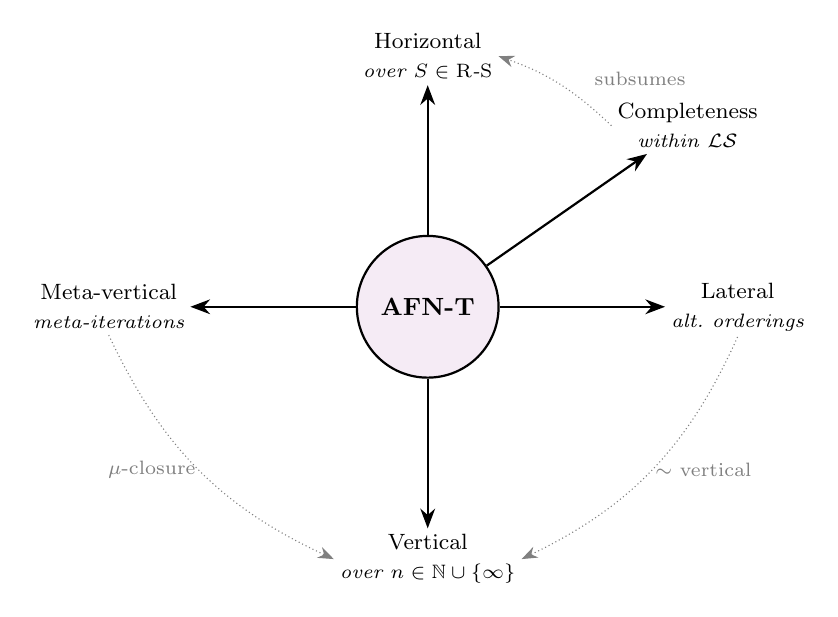
\begin{tikzpicture}[
  axis/.style={-{Stealth[length=2.5mm]}, thick},
  dep/.style={-{Stealth[length=2mm]}, thin, gray, densely dotted},
  label/.style={font=\footnotesize, align=center, inner sep=2pt},
  center/.style={draw, circle, thick, minimum size=1.8cm, align=center, font=\bfseries\small, fill=violet!8}
]
\node[center] (C) at (0,0) {AFN-T};
\node[label, above=1.9cm of C]          (H) {Horizontal \\[1pt] \scriptsize\itshape over $S \in \RS$};
\node[label, below=1.9cm of C]          (V) {Vertical \\[1pt] \scriptsize\itshape over $n \in \mathbb{N} \cup \{\infty\}$};
\node[label, left=2.1cm of C]           (M) {Meta-vertical \\[1pt] \scriptsize\itshape meta-iterations};
\node[label, right=2.1cm of C]          (L) {Lateral \\[1pt] \scriptsize\itshape alt.\ orderings};
\node[label] (K) at (3.3,2.3) {Completeness \\[1pt] \scriptsize\itshape within $\cL\cS$};
\draw[axis] (C) -- (H);
\draw[axis] (C) -- (V);
\draw[axis] (C) -- (M);
\draw[axis] (C) -- (L);
\draw[axis] (C) -- (K);
\draw[dep] (K.west) to[bend right=12] node[pos=0.35, above right=2pt and 6pt, font=\scriptsize, text=gray, inner sep=1pt] {subsumes} (H.east);
\draw[dep] (L.south) to[bend left=20] node[midway, right, font=\scriptsize, text=gray, inner sep=1pt] {$\sim$ vertical} (V.east);
\draw[dep] (M.south) to[bend right=20] node[midway, left, font=\scriptsize, text=gray, inner sep=1pt] {$\mu$-closure} (V.west);
\end{tikzpicture}
\caption{Five-axis absoluteness of AFN-T (Theorems~\ref{thm:horizontal}--\ref{thm:completeness}). Solid arrows are the five axes along which AFN-T is absolute: horizontal (Theorem~\ref{thm:horizontal}), vertical (Theorem~\ref{thm:vertical}), meta-vertical (Theorem~\ref{thm:meta-vertical}), lateral (Theorem~\ref{thm:lateral}), and --- conditional on Lawvere-scope --- completeness (Theorem~\ref{thm:completeness}). Dotted arrows mark the structural dependencies established in: the completeness axis subsumes the horizontal one; the lateral axis reduces to the vertical one via Ara--Maltsiniotis and Barwick--Schommer-Pries; and the meta-vertical axis is the $\mu$-closure of the vertical axis under $(\infty, \infty)$-stabilization. A minimal logically independent presentation features only horizontal and vertical.}
\label{fig:five-axis}
\end{figure}

\begin{theorem}[Horizontal absoluteness]\label{thm:horizontal}
AFN-T (Theorem~\ref{thm:afnt-alpha}) holds for every $S \in \RS$ uniformly: there is a single proof working for all Rich-metatheories satisfying (R1)--(R5).
\end{theorem}

\begin{proof}
The proof of Theorem~\ref{thm:afnt-alpha} consists of a single application of Lemma~\ref{lem:SS-membership} (syntax--semantics bridge) together with the observation that $\id_X : X \to X$ realizes a Morita reduction violating $(\Pi_{4, S, n})$. Lemma~\ref{lem:SS-membership} uses only (R1), (R2), (R5a) (for the Grothendieck-construction identification of $\Syn(F)$ as an $S$-definable $(\infty, n_F)$-category); the Morita-reduction observation uses only the categorical identity morphism. No datum from $S$ beyond (R1)--(R5) is invoked. Hence the proof applies uniformly to all $S \in \RS$.
\end{proof}

\begin{theorem}[Vertical absoluteness]\label{thm:vertical}
AFN-T (Theorem~\ref{thm:afnt-alpha}) holds for every categorical level $n \in \mathbb{N} \cup \{\infty\}$.
\end{theorem}

\begin{proof}
The syntax--semantics bridge of Theorem~\ref{thm:afnt-alpha} relies on (R5a) through Lemma~\ref{lem:SS-membership}: $\Syn(F)$ is an $S$-definable $(\infty, n_F)$-category for every $n$. The Lambek--Scott adjunction holds uniformly for all $(\infty, n)$-levels (classical for $n = 0, 1$; Lurie~\cite{LurieHTT} \S 5--\S 6 for $n = 1$; for general $(\infty, n)$, via Barwick--Schommer-Pries~\cite{BarwickSchommerPries2021} with Bergner--Rezk~\cite{BergnerRezk2013} model comparison).

For the limit $n = \infty$: $\Syn(F)$ stabilizes via
\[ (\infty, \infty)\text{-}\Cat = \colim_{n < \infty} (\infty, n)\text{-}\Cat, \]
and the identification of $\Syn(F)$ as an $S$-definable derived construction is preserved at the limit. The Morita reduction $\id_X : X \to X$ is the categorical identity morphism and transfers trivially to any $(\infty, n)$-level.
\end{proof}

\begin{theorem}[Meta-vertical stabilization]\label{thm:meta-vertical}
At the categorical level $(\infty, \infty)$, any meta-iteration of the above types stabilizes: $(\infty, \infty + 1)\text{-}\Cat = (\infty, \infty)\text{-}\Cat$. Therefore, meta-iterations do not escape AFN-T.
\end{theorem}

\begin{proof}
By the unicity theorem of Barwick--Schommer-Pries~\cite{BarwickSchommerPries2021} together with the model comparisons of Bergner--Rezk~\cite{BergnerRezk2013} and Ara--Maltsiniotis~\cite{AraMaltsiniotis2017}, the tower of $(\infty, n)$-categories stabilizes at $n = \infty$: further iteration adds no new structure. Specifically, the canonical inclusion
\[ (\infty, \infty)\text{-}\Cat \hookrightarrow (\infty, \infty + 1)\text{-}\Cat \]
is an equivalence.

For iterated functor categories: $\Fun^k(\cC) \subseteq (\infty, \infty)\text{-}\Cat$ for any $k$; the limit is again $(\infty, \infty)$-$\Cat$.

For non-standard models: these require either (a) enriching the theory beyond R-S (violating (R2)), or (b) reducing through Aczel anti-foundation axiom (AFA) to standard non-well-founded sets (Aczel~\cite{Aczel1988}), which does not add structural axes.

Therefore, all meta-iterations stabilize within the existing five axes.
\end{proof}

\begin{theorem}[Lateral absoluteness]\label{thm:lateral}
All alternative categorical orderings reduce to (or enrich) the $(\infty, n)$-hierarchy and therefore satisfy AFN-T.
\end{theorem}

\begin{proof}
Each listed ordering admits a canonical translation to $(\infty, n)$-$\Cat$ for appropriate $n$:
\begin{itemize}
\item Operads $\to$ symmetric monoidal $(\infty, 1)$-categories (Lurie HA~\cite{LurieHA} \S 5).
\item Double categories $\to$ $(\infty, 2)$-categories (Grandis).
\item Globular/cubical/opetopic $\omega$-categories $\simeq (\infty, \infty)$-categories (Ara--Maltsiniotis~\cite{AraMaltsiniotis2017}).
\item Stable $(\infty, 1)$-categories $\to (\infty, 1)$-categories via spectrification.
\item Fusion categories $\to$ finite $(\infty, 1)$-categories.
\end{itemize}
In each case, the translation preserves formal definability: objects in the alternative ordering correspond to objects in the $(\infty, n)$-hierarchy at the relevant level. Therefore, AFN-T applies uniformly across all orderings.
\end{proof}

\begin{definition}[Lawvere-scope]\label{def:law-scope}
A foundational theory $F$ belongs to the \textbf{Lawvere-scope} $\cL\cS$ if the following structural properties hold (the metatheory in which $\Syn(F)$ and $\Mod(F)$ are constructed is arbitrary but fixed throughout the four clauses):
\begin{itemize}
\item \textbf{(L1)} $F$ has a syntactic category $\Syn(F)$ --- a small category of contexts and provable substitutions.
\item \textbf{(L2)} $F$ has a semantic $2$-category $\Mod(F)$ --- the $2$-category of models.
\item \textbf{(L3)} There exists a canonical adjunction $\Syn \dashv \Mod$ (Lawvere~\cite{Lawvere1969}).
\item \textbf{(L4)} $\Mod(F)$ is realizable as an $(\infty, n)$-category for some $n$ (Grothendieck--Lurie tradition).
\end{itemize}
Membership in $\cL\cS$ is a structural property of $F$ and does not presuppose any specific R-S. In particular, every R-S $S$ is itself in $\cL\cS$ (take the tautological $\Syn = S$, $\Mod = \Mod(S)$ from (R5)), so the notion is circularity-free for the application in Theorem~\ref{thm:completeness}.
\end{definition}

\begin{theorem}[Completeness axis, conditional on Lawvere-scope]\label{thm:completeness}
Suppose $F \in \cL\cS$. Then every structural variation of $F$ reduces to one of the four axes (horizontal, vertical, meta-vertical, lateral). In particular, AFN-T is five-axis absolute within $\cL\cS$.
\end{theorem}

\begin{proof}
Let $F \in \cL\cS$. By Definition~\ref{def:law-scope}, $F$ is characterized by a quadruple:
\begin{itemize}
\item \textbf{(A) Syntactic structure $\Syn(F)$}: signature + axioms + inference rules --- the \emph{horizontal axis} (over R-S).
\item \textbf{(B) Semantic depth}: the level $n$ of $\Mod(F)$ as $(\infty, n)$-category --- the \emph{vertical axis}.
\item \textbf{(C) Meta-reflection}: iterations of G\"odel coding and reflection principles --- the \emph{meta-vertical axis}.
\item \textbf{(D) Alternative semantics}: operadic, globular, cubical, opetopic, etc.\ --- the \emph{lateral axis}.
\end{itemize}
Thus any putative fifth axis $\eta$ must, by the Lawvere characterization, be a subcomponent of one of (A)--(D). Either $\eta \subseteq$ (A), in which case AFN-T for $\eta$ reduces to horizontal absoluteness (Theorem~\ref{thm:horizontal}); $\eta \subseteq$ (B), reducing to vertical (Theorem~\ref{thm:vertical}); $\eta \subseteq$ (C), reducing to meta-vertical (Theorem~\ref{thm:meta-vertical}); or $\eta \subseteq$ (D), reducing to lateral (Theorem~\ref{thm:lateral}). There is no independent fifth axis within $\cL\cS$.
\end{proof}

\section{Three Standard Bypass Paths}\label{sec:bypass}

\begin{theorem}[Universe polymorphism absoluteness]\label{thm:universe}
Universe-polymorphic structures in any Rich-metatheory $S$ are Morita-reducible to derived constructions over the $(\infty, 1)$-topos of small categories. Formally: if $X$ is specified as
\[ X = \prod_{\ell : \mathrm{Level}} F(\ell) \]
for a family of functors $F(\ell) : \cU_\ell \to \cU_\ell$, then
\[ X \simeq \lim_\ell \Fun(\cU_\ell, \cU_\ell) \in \cS_S^{\mathrm{global}}. \]
In particular, $X \in \cS_S$, and universe-polymorphic structures satisfy $\neg (\Pi_4)$.
\end{theorem}

\begin{proof}
A universe-polymorphic structure $X = \prod_\ell F(\ell)$ is a section of the Grothendieck fibration $\pi : \int \cU \to \mathrm{Level}$, where $\cU_\ell$ is the universe at level $\ell$. By standard Grothendieck construction theory (Lurie HTT~\cite{LurieHTT} \S 3.2), sections of this fibration correspond to functors $\mathrm{Level} \to \int \cU$, and the space of such sections is
\[ \Gamma(\pi) = \lim_\ell \Fun(\cU_\ell, \cU_\ell). \]
This is a derived construction (an indexed limit), hence belongs to $\cS_S^{\mathrm{global}}$.

For $(\infty, n)$-versions: the construction extends via Lurie HTT \S 4.2 (limits in $(\infty, n)$-categories).
\end{proof}

\[ S_{\kappa+1} = S_\kappa + \Con(S_\kappa) \]
and hopes that the limit $S_\infty$ captures something beyond its starting point.

\begin{theorem}[Reflective tower boundedness]\label{thm:reflective}
For every Rich-metatheory $S$, the reflective tower $\{S_\kappa\}$ stabilizes at an inaccessible cardinal bound:
\[ \Con(\text{reflective tower over }S) = \Con(S) + \kappa_{\mathrm{inacc}}, \]
exactly one additional inaccessible cardinal. No $\LAbs$ escape occurs through this path.
\end{theorem}

\begin{proof}
The proof uses two results.

\textbf{Step 1} (upper bound). The tower $\{S_\kappa\}$ has proof-theoretic ordinal bounded by the first inaccessible cardinal over $S$. This follows from the standard analysis of reflection principles: the reflection principle $\Con(S)$ adds at most one inaccessible cardinal to the consistency strength of $S$ (Rathjen~\cite{Rathjen1999}, Feferman~\cite{Feferman1964}).

\textbf{Step 2} (stabilization). By the $(\infty, \infty)$-meta-vertical stabilization (Theorem~\ref{thm:meta-vertical}), the tower does not extend indefinitely at the categorical level: $(\infty, \infty + 1)\text{-}\Cat = (\infty, \infty)\text{-}\Cat$.

Combining: the tower is bounded above by $\Con(S) + \kappa_{\mathrm{inacc}}$ and stabilizes at the $(\infty, \infty)$-level. Any limit $S_\infty$ remains within the Lawvere-scope and within $\cS_S$.
\end{proof}

This is the most subtle of the three bypass paths, as intensional refinement genuinely refines the base-level classification. I address it in detail through the construction of the intensional refinement functor $\II$ and the proof of its slice-locality.

I begin by defining the target $2$-category of display $2$-categories.

\begin{definition}[Display $2$-class]\label{def:display-class}
Let $\cC$ be a $2$-category with $2$-pullbacks. A \textbf{display class} $\cD \subseteq \Mor_1(\cC)$ is a class of $1$-morphisms satisfying:
\begin{itemize}
\item \textbf{(D1) Contains equivalences}: every $1$-equivalence in $\cC$ lies in $\cD$.
\item \textbf{(D2) Pullback-stable}: for $d : B \to A$ in $\cD$ and any $f : A' \to A$, the $2$-pullback $f^*d : f^*B \to A'$ exists and lies in $\cD$.
\item \textbf{(D3) Closed under composition}: if $d_1 : C \to B \in \cD$ and $d_2 : B \to A \in \cD$, then $d_2 \circ d_1 \in \cD$.
\item \textbf{(D4) $2$-cell coherent}: for a $2$-morphism $\phi : f \Rightarrow g : A' \to A$ and $d \in \cD$, the induced $2$-morphism $\phi^* d : f^* d \Rightarrow g^* d$ is an isomorphism in the slice over $A'$.
\end{itemize}
\end{definition}

\begin{definition}[Display $2$-category]\label{def:display-2-cat}
A \textbf{display $2$-category} is a triple $(\cC, \cD, \iota)$ where:
\begin{itemize}
\item $\cC$ is a locally small $2$-category with $2$-pullbacks.
\item $\cD$ is a display class in $\cC$.
\item $\iota : \cD \hookrightarrow \Mor_1(\cC)$ is the canonical inclusion.
\end{itemize}
\end{definition}

\begin{definition}[The $2$-category $\Sint$]\label{def:Sint}
The $2$-category $\Sint$ of display $2$-categories has:
\begin{itemize}
\item \textbf{Objects}: display $2$-categories $(\cC, \cD, \iota)$.
\item \textbf{$1$-morphisms}: pairs $(F, F_\cD) : (\cC_1, \cD_1, \iota_1) \to (\cC_2, \cD_2, \iota_2)$ where $F : \cC_1 \to \cC_2$ is a $2$-functor and $F_\cD : \cD_1 \to \cD_2$ is a restriction of $F$, such that $F \circ \iota_1 = \iota_2 \circ F_\cD$ and $2$-pullbacks are preserved up to coherent $2$-isomorphisms.
\item \textbf{$2$-morphisms}: natural $2$-transformations $\eta : F \Rightarrow G$ whose restrictions $\eta|_\cD : F_\cD \Rightarrow G_\cD$ are coherently aligned.
\end{itemize}
\end{definition}

\begin{theorem}[Existence of $\II$]\label{thm:I-existence}
There exists a contravariant $2$-functor
\[ \II : \cF^{\mathrm{op}} \to \Sint \]
from the $2$-category of Rich-foundations ($\LFnd$) to $\Sint$, with the following properties:
\begin{enumerate}
\item[\textbf{(I-1)}] \textbf{Homotopy invariance}: every $2$-equivalence $\phi : f \simeq g$ in $\cF$ induces a $2$-isomorphism $\II(\phi) : \II(f) \simeq \II(g)$ in $\Sint$.
\item[\textbf{(I-2)}] \textbf{Gauge covariance}: for a gauge transformation $\tau : F_1 \to F_2$, $\II(\tau) : \II(F_2) \to \II(F_1)$ is a $1$-morphism in $\Sint$, and is a $1$-equivalence when $\tau$ is invertible.
\item[\textbf{(I-3)}] \textbf{Strict refinement of Morita}: there exist $F_1, F_2 \in \cF$ with $F_1 \sim_M F_2$ (Morita equivalent) but $\II(F_1) \not\simeq \II(F_2)$.
\item[\textbf{(I-4)}] \textbf{Morita as $2$-localization}: the forgetful $2$-functor $\cU : \Sint \to 2\text{-}\Cat$, $(\cC, \cD, \iota) \mapsto \cC$, satisfies $\cU \circ \II \simeq \rho$ (the classification functor); Morita equivalence is recovered through $2$-localization of $\II$ by the class $\mathcal{W}_\cU = \cU^{-1}(1\text{-equiv}(2\text{-}\Cat))$.
\end{enumerate}
\end{theorem}

\begin{proof}

\textbf{Step 1} (construction on objects). For $F \in \cF$, I construct $\II(F) = (\cC_F, \cD_F, \iota_F) \in \Ob(\Sint)$:
\begin{itemize}
\item $\cC_F := \cF / F$ is the slice $2$-category: objects are pairs $(F', p : F' \to F)$; $1$-morphisms are coherent triangles over $F$; $2$-morphisms are $2$-cells compatible with the projection to $F$.
\item $\cD_F$ is the \textbf{canonical minimal display class}: the smallest class of $1$-morphisms in $\cC_F$ containing all $1$-equivalences and closed under $2$-pullbacks, composition, and $2$-cells. Formally,
\[ \cD_F := \bigcap \{\cD' \subseteq \Mor_1(\cC_F) : \cD' \text{ is a display class containing all } 1\text{-equivalences}\}. \]
This intersection is non-empty (it contains the class of all $1$-morphisms) and is itself a display class by closure-of-intersections arguments.

\textbf{Explicit description of $\cD_F$ via inductive construction}:
\begin{itemize}
\item $\cD_F^{(0)}$: all $1$-equivalences.
\item $\cD_F^{(n+1)}$: objects obtained from $\cD_F^{(n)}$ by $2$-pullback along arbitrary morphisms, composition of elements in $\cD_F^{(n)}$, or transport along $2$-cells.
\item $\cD_F := \bigcup_{n < \omega} \cD_F^{(n)}$.
\end{itemize}
This definition produces a class automatically satisfying (D1)--(D4) by construction, without requiring the ambient $\cC_F$ to be locally cartesian closed or to have exponentials.

\item $\iota_F : \cD_F \hookrightarrow \Mor_1(\cC_F)$ is the canonical inclusion.
\end{itemize}

\textbf{Step 2} (construction on $1$-morphisms). For $f : F_1 \to F_2$ in $\cF$, define
\[ \II(f) := (f^*, f^*|_\cD) : (\cF / F_2, \cD_{F_2}, \iota_{F_2}) \to (\cF / F_1, \cD_{F_1}, \iota_{F_1}) \]
where $f^* : \cF / F_2 \to \cF / F_1$ is the pullback $2$-functor. The direction is contravariant: $\II$ takes $f$ to a $1$-morphism in the opposite direction.

That $f^*$ preserves display-class elements follows by induction on the class generation: base class is $1$-equivalences, which are preserved by pullback; inductive closure steps are preserved by pullback by the pullback-of-pullback property.

\textbf{Step 3} (construction on $2$-morphisms). For $\phi : f \Rightarrow g$ in $\cF$, the induced natural $2$-transformation $\phi^* : f^* \Rightarrow g^*$ (Beck--Chevalley structure) restricts coherently to display classes by (D4). This yields
\[ \II(\phi) : \II(f) \Rightarrow \II(g) \]
in $\Sint$.

\textbf{Step 4} (functoriality). $\II(\id_F) = \id_{\II(F)}$ is immediate. $\II(g \circ f) \simeq \II(f) \circ \II(g)$ follows from the Beck--Chevalley coherence of pullback composition.

\textbf{Step 5} (verification of (I-1)). A $2$-equivalence $\phi : f \simeq g$ has a $2$-inverse $\phi^{-1}$. The induced $\phi^* : f^* \Rightarrow g^*$ is invertible via $(\phi^{-1})^*$. Therefore, $\II(\phi)$ is a $2$-isomorphism in $\Sint$.

\textbf{Step 6} (verification of (I-2)). For a gauge transformation $\tau : F_1 \to F_2$ (a $1$-morphism with a distinguished $2$-equivalence of $\rho$-projections), the pullback $\tau^*$ induces $\II(\tau) : \II(F_2) \to \II(F_1)$. If $\tau$ is invertible, $\II(\tau)$ is a $1$-equivalence by Step 5.

\textbf{Step 7} (verification of (I-3)). I exhibit the classical extensional-collapse example.

\emph{Computability framework.} To state the invariant $\tau$ precisely I fix a computability model: I work inside the \emph{effective topos} $\mathrm{Eff}$ (Hyland~\cite{Hyland1982}), regarded as the reference internal model of constructive computability. All $2$-functors and $2$-equivalences in the sub-$2$-category $\Sint^{\mathrm{eff}} \subseteq \Sint$ are required to be internally computable in $\mathrm{Eff}$; equivalently, both the functor and its quasi-inverse are realized by recursive morphisms. This restriction is conservative for the argument below because the Morita equivalence of Hofmann~\cite{Hofmann1995} is constructed explicitly through primitive-recursive translations and hence lies in $\Sint^{\mathrm{eff}}$.

Let $F_1 := \MLTT$ (Martin-L\"of type theory with propositional identity types) and $F_2 := \ETT$ (extensional type theory with definitional equality reflection).

\emph{Morita equivalence}: $F_1 \sim_M F_2$ is established by Hofmann~\cite{Hofmann1995} (conservativity theorem, Chapter 3): the categories of models of $\MLTT + \mathsf{UIP}$ and of $\ETT$ are equivalent on the class of reasonable cartesian closed categories.

\emph{Intensional distinction}: define the typing invariant $\tau : \Ob(\Sint^{\mathrm{eff}}) \to \{0, 1\}$ by
\[ \tau(\cC, \cD, \iota) := \begin{cases} 1 & \text{if there exists an $\mathrm{Eff}$-internal normalization procedure for all } d \in \cD, \\ 0 & \text{otherwise.} \end{cases} \]

The invariant $\tau$ is a $2$-invariant of $\Sint^{\mathrm{eff}}$-equivalence: any computable $2$-equivalence $(F, F_\cD) : (\cC_1, \cD_1) \simeq (\cC_2, \cD_2)$ in $\Sint^{\mathrm{eff}}$ transfers the normalization procedure along the realizer for $F_\cD^{-1}$. The computability restriction is essential: without it, an abstract $2$-equivalence could, in principle, identify a normalizing with a non-normalizing display class via a non-computable bijection. Within $\mathrm{Eff}$, no such bijection exists as an internal morphism.

Applying to $\II(F_1), \II(F_2)$:
\begin{itemize}
\item $\tau(\II(F_1)) = 1$: $\MLTT$ has strongly normalizing typechecking (Streicher~\cite{Streicher1991} Theorem 3.3; Werner~\cite{Werner1994}).
\item $\tau(\II(F_2)) = 0$: $\ETT$ with reflection rule has undecidable typechecking (Hofmann~\cite{Hofmann1995}, Chapter 3), and no $\mathrm{Eff}$-internal normalizer exists.
\end{itemize}

Therefore $\tau(\II(F_1)) \neq \tau(\II(F_2))$, so $\II(F_1) \not\simeq \II(F_2)$ in $\Sint^{\mathrm{eff}}$, despite $F_1 \sim_M F_2$.

\textbf{Step 8} (verification of (I-4)). For $F \in \cF$,
\[ \cU(\II(F)) = \cC_F = \cF / F. \]
By the $2$-categorical Yoneda lemma (Kelly~\cite{Kelly1982} Theorem 2.4.1), $\cF / F \simeq \rho(F)$ up to $2$-equivalence. Thus $\cU \circ \II \simeq \rho$.

For the Morita $2$-localization: define
\[ \mathcal{W}_\cU := \{(F, F_\cD) \in \Mor_1(\Sint) : F \in 1\text{-equiv}(2\text{-}\Cat)\}. \]
The class $\mathcal{W}_\cU$ satisfies the $2$-calculus-of-fractions conditions (Pronk~\cite{Pronk1996}, Kelly--Street~\cite{KellyStreet1974}): $2$-closure under composition, containing identities, compatibility with $2$-pullbacks. By Pronk's theorem, the $2$-localization $\Sint[\mathcal{W}_\cU^{-1}]$ exists with the universal property:
\[ \Sint[\mathcal{W}_\cU^{-1}] \simeq \image(\cU)_{\mathrm{gauge}} = \fM \]
(the last equivalence following from the gauge identification of $\fM$ as $\Trace(\mathsf{A})/\mathrm{gauge}$ in the moduli stack sense).

Thus Morita equivalence is recovered from $\II$ through $2$-localization.
\end{proof}

\begin{theorem}[Slice-locality of $\II$]\label{thm:slice-locality}
Let $\II : \cF^{\mathrm{op}} \to \Sint$ be the functor from Theorem~\ref{thm:I-existence}, and let $\pi : \cF \to \fM$ be the gauge quotient. Then:
\begin{enumerate}
\item[\textbf{(a)}] There exists a $2$-functor $\tpi : \Sint \to \fM$ making the diagram
\[
\begin{tikzcd}
\cF \arrow[r, "\II"] \arrow[d, "\pi"'] & \Sint \arrow[d, "\tpi"] \\
\fM \arrow[r, equal] & \fM
\end{tikzcd}
\]
$2$-commute.
\item[\textbf{(b)}] The fiber $\tpi^{-1}([F])$ over a point $[F] \in \fM$ is a $2$-category $\mathrm{Int}([F])$, the \emph{intensional layer over the gauge class}.
\item[\textbf{(c)}] Intensional refinement does not produce new points in $\fM$: for every object $X$ in the image of $\II$, $\tpi(X) \in \fM$ is an already-existing point.
\end{enumerate}
\end{theorem}

\begin{proof}

\textbf{(a)} Define $\tpi := [\, \cdot \,]_{\mathrm{gauge}} \circ \cU$, where $[\, \cdot \,]_{\mathrm{gauge}} : 2\text{-}\Cat \to \fM$ is the gauge quotient on ambient $2$-categories. By (I-4), $\tpi \circ \II = [\rho(\cdot)]_{\mathrm{gauge}} = \pi$, since gauge classes of $F$ and $\rho(F)$ coincide by definition.

\textbf{(b)} For $[F] \in \fM$,
\[ \mathrm{Int}([F]) := \tpi^{-1}([F]) = \{(\cC, \cD, \iota) \in \Sint : [\cC]_{\mathrm{gauge}} = [F]_{\mathrm{gauge}}\}. \]
This is a full $2$-subcategory of $\Sint$: its $2$-morphisms are inherited. The non-triviality of $\mathrm{Int}([F])$ follows from (I-3): $\II(\MLTT)$ and $\II(\ETT)$ lie in $\mathrm{Int}([\MLTT])$ but are non-equivalent.

The $2$-fibration structure: for $[F] \in \fM$ and $f : [F'] \to [F]$, cartesian lift exists through $2$-pullback in $\Sint$; cartesian lifts compose up to coherent $2$-iso (standard Grothendieck $2$-fibration theory; Hermida~\cite{Hermida1999}, Bakovic~\cite{Bakovic2010}).

\textbf{(c)} For $\alpha_{\mathrm{new}} \in \image(\II)$, $\alpha_{\mathrm{new}} = \II(F)$ for some $F \in \cF$. Then $\tpi(\alpha_{\mathrm{new}}) = \pi(F) = [F]_{\mathrm{gauge}} \in \fM$ --- an existing point. No new base point is produced.
\end{proof}

\begin{corollary}[Intensional refinement is slice-level]\label{cor:slice-level}
Intensional refinement adds no new structural axis to AFN-T: the base ($\fM$) is untouched, and TH-absoluteness holds without modification.
\end{corollary}

\begin{proof}
Five-axis absoluteness (Theorems~\ref{thm:horizontal}--\ref{thm:completeness}) concerns points of $\fM$. Theorem~\ref{thm:slice-locality}(c) shows intensional refinement acts only on fibers, not base points. No new axis of variation is introduced.
\end{proof}

\section{\texorpdfstring{$\LCls$ Meta-Classification}{Classifier Meta-Classification}}\label{sec:meta}

\subsection{\texorpdfstring{The Class $\Meta_{\mathrm{Cls}}$}{The Class Meta\_5+}}

\begin{definition}[$\LCls$ meta-structure]\label{def:meta}
An object $\mathbf{F}$ is a \textbf{$\LCls$ meta-structure} if it satisfies:
\begin{itemize}
\item \textbf{(M1) Locally small $2$-category}: $\mathbf{F}$ is a locally small $2$-category.
\item \textbf{(M2) Classification functor}: there is a $2$-functor $\Cl_{\mathbf{F}} : \mathbf{F} \to \fM(\mathbf{F}) \subseteq \fM$, where $\fM(\mathbf{F})$ is some classifying $2$-stack of Rich-foundations.
\item \textbf{(M3) Accessible reflection}: there is an accessible endofunctor $R_{\mathbf{F}} : \mathbf{F} \to \mathbf{F}$.
\item \textbf{(M4) Non-generative}: $\mathbf{F}$ does not derive the axioms of foundations $F \in \image(\Cl_{\mathbf{F}})$ from its own axioms; classification is parametric, not axiomatic.
\item \textbf{(M5) Metatheory-parametrized}: $\mathbf{F}$ is defined within some $S \in \RS$.
\end{itemize}
I denote the class of such $\mathbf{F}$ as $\Meta_{\mathrm{Cls}}$.
\end{definition}

\begin{definition}[Maximality]\label{def:maximality}
A meta-structure $\mathbf{F} \in \Meta_{\mathrm{Cls}}$ is \textbf{maximal} if additionally:
\begin{itemize}
\item \textbf{(Max-1) Full classification}: $\image(\Cl_{\mathbf{F}}) = \fM$.
\item \textbf{(Max-2) Gauge-fullness}: $\mathrm{Aut}_2(\mathbf{F})$ acts transitively on gauge classes in $\image(\Cl_{\mathbf{F}})$.
\item \textbf{(Max-3) Depth stratification}: $\mathbf{F}$ admits a \emph{depth-indexed filtration} $\mathbf{F}^{(0)} \hookrightarrow \mathbf{F}^{(1)} \hookrightarrow \cdots \hookrightarrow \mathbf{F}^{(n)} \hookrightarrow \cdots$ of accessible $2$-subcategories with $\mathbf{F} \simeq_2 \colim_{n < \omega} \mathbf{F}^{(n)}$, equipped with a \emph{depth function} $\dep : \Ob(\mathbf{F}) \to \omega$ assigning to each object the least $n$ such that the object lies in $\mathbf{F}^{(n)}$, satisfying the following \emph{predicativity condition}: for every predicate $P$ appearing in a definition by comprehension of an object $A \in \mathbf{F}^{(n)}$ (i.e., the definition has the form ``$A :=$ the object classifying $\{x : P(x)\}$''), every object $Y$ that appears as the target of a sub-expression in $P$ --- in particular every target of $R_\mathbf{F}$, $\Cl_\mathbf{F}$, or subobject-classifier evaluations --- satisfies $\dep(Y) < n$.
\item \textbf{(Max-4) Intensional completeness}: there exists a $2$-functor $\II_{\mathbf{F}} : \mathbf{F}^{\mathrm{op}} \to \Sint$ satisfying properties (I-1)--(I-4) of Theorem~\ref{thm:I-existence}.
\end{itemize}
I denote the class of maximal meta-structures as $\Meta_{\mathrm{Cls}}^{\top}$.
\end{definition}

\subsection{Meta-Categoricity}

\begin{theorem}[Meta-Categoricity]\label{thm:meta-cat}
Let $\mathbf{F}_1, \mathbf{F}_2 \in \Meta_{\mathrm{Cls}}^{\top}$ be parametrized by the same Rich-metatheory $S \in \RS$. Then $\mathbf{F}_1 \simeq_{(\infty, \infty)} \mathbf{F}_2$ via a canonical equivalence.
\end{theorem}

\begin{proof}
I show that each $\mathbf{F}_i$ is canonically $(\infty, \infty)$-equivalent to a common object $\mathbf{F}_S^*$ constructed from $S$, whence $\mathbf{F}_1 \simeq_{(\infty, \infty)} \mathbf{F}_S^* \simeq_{(\infty, \infty)} \mathbf{F}_2$.

\textbf{Step 1: the canonical maximal classifier.} Let $\rho : \cF \to (\infty, n_S)\text{-}\Cat$ be the classification functor of Convention~\ref{conv:notation}. Consider the Grothendieck straightening applied to the Cartesian fibration $\int \rho \to S$, with gauge-quotient:
\[ \mathbf{F}_S^* := \mathbf{St}(\rho) / \mathrm{gauge}, \]
where $\mathbf{St}(\rho)$ is the straightening of $\rho$.

\textbf{Step 2: construction of $\Phi_\mathbf{F}$.} Any $\mathbf{F} \in \Meta_{\mathrm{Cls}}^{\top}$ carries four structures: a classification functor $\Cl_{\mathbf{F}} : \mathbf{F} \to \fM$ essentially surjective onto $\fM$ by (Max-1); a transitive $\mathrm{Aut}_2$-action on gauge classes by (Max-2); a canonical depth filtration $\mathbf{F}^{(\bullet)}$ by (Max-3); a canonical intensional completion $\II_{\mathbf{F}} : \mathbf{F}^{\mathrm{op}} \to \Sint$ with (I-1)--(I-4) by (Max-4).

Each structure admits a universal presentation on $\mathbf{F}_S^*$: classification is identity on $\fM$; gauge is canonical; the depth filtration is $\mathbf{F}_S^{*(n)} := \{[\alpha] : \dep_S^*([\alpha]) < n\}$ with $\dep_S^*([\alpha])$ the quantifier-rank of the defining formula of $F_{[\alpha]}$ in $\Syn(S)$ (finite by (R2), (F-3); (Max-3) predicativity follows by Kleene arithmetic-hierarchy induction); $\II_{\mathbf{F}_S^*}$ is the Yoneda embedding factoring through $\tilde\pi$ (Theorem~\ref{thm:slice-locality}). By the universal property of Grothendieck straightening (Lurie HTT~\cite{LurieHTT} Theorem 3.2.0.1) in $\mathbf{StrCat}_{S, 2}$, there exists a unique (up to canonical $(\infty, 2)$-isomorphism) $2$-functor
\[ \Phi_\mathbf{F} : \mathbf{F} \to \mathbf{F}_S^* \]
preserving all four structures.

\textbf{Step 3: $\Phi_\mathbf{F}$ is essentially surjective.} For every gauge-class $[\alpha] \in \fM$, (Max-1) gives $A \in \mathbf{F}$ with $\Cl_\mathbf{F}(A) = [\alpha]$, and $\Phi_\mathbf{F}(A)$ projects to the same class in $\mathbf{F}_S^*$. Transitivity of the $\mathrm{Aut}_2(\mathbf{F})$-action on gauge classes (Max-2) ensures this covers all of $\mathbf{F}_S^*$.

\textbf{Step 4: $\Phi_\mathbf{F}$ is fully faithful.} I prove that for every $A, B \in \mathbf{F}$ the induced map
\[ \Phi_\mathbf{F} : \Hom_\mathbf{F}(A, B) \longrightarrow \Hom_{\mathbf{F}_S^*}(\Phi_\mathbf{F}(A), \Phi_\mathbf{F}(B)) \]
is an equivalence of Hom-spaces.

\emph{Faithfulness}: suppose $f, g : A \to B$ in $\mathbf{F}$ have $\Phi_\mathbf{F}(f) = \Phi_\mathbf{F}(g)$. Applying $\Cl_\mathbf{F}$ to both sides yields $\Cl_\mathbf{F}(f) = \Cl_\mathbf{F}(g)$ in $\fM$, so $f$ and $g$ differ at most by gauge. Applying $\II_\mathbf{F}$ (which satisfies (I-1) homotopy invariance and (I-2) gauge covariance of Theorem~\ref{thm:I-existence}), $\II_\mathbf{F}(f) = \II_\mathbf{F}(g)$ in $\Sint$. By (I-3) strict refinement of Morita and (I-4) Morita-as-$2$-localization, $\II_\mathbf{F}$ is jointly faithful with $\Cl_\mathbf{F}$: the pair $(\Cl_\mathbf{F}, \II_\mathbf{F})$ separates morphisms in $\mathbf{F}$. Hence $f = g$.

\emph{Fullness}: given $h : \Phi_\mathbf{F}(A) \to \Phi_\mathbf{F}(B)$ in $\mathbf{F}_S^*$, I lift $h$ to $\mathbf{F}$. The morphism $h$ factors as $h_{\mathrm{ext}} \in \Hom_\fM(\Cl_\mathbf{F}(A), \Cl_\mathbf{F}(B))$ (extensional part, via the canonical projection $\mathbf{F}_S^* \to \fM$) together with $h_{\mathrm{int}} \in \Hom_{\Sint}(\II_{\mathbf{F}_S^*}(B), \II_{\mathbf{F}_S^*}(A))$ (intensional fiber, via $\II_{\mathbf{F}_S^*}$). By (Max-1), $h_{\mathrm{ext}}$ lifts to a gauge-class of morphisms $A \to B$ in $\cF$ at the classified level; (Max-2) transitivity picks a representative in $\mathbf{F}$. By (Max-4), $h_{\mathrm{int}}$ lifts uniquely to the intensional completion of $\mathbf{F}$, which by (I-4) Morita-as-$2$-localization coincides with the intensional data of $\II_\mathbf{F}$. Combining, I obtain a morphism $\tilde h : A \to B$ in $\mathbf{F}$ with $\Phi_\mathbf{F}(\tilde h) = h$.

\emph{$2$-morphisms}: the same argument applied one dimension up --- using (M3) accessibility of the reflection and (Max-4) intensional $2$-functoriality --- establishes the Hom-equivalence at the level of $2$-cells. The full coherent $(\infty, 2)$-equivalence follows by induction on truncation levels.

Hence $\Phi_\mathbf{F}$ is a $2$-equivalence in $\mathbf{StrCat}_{S, 2}$.

\textbf{Step 3: lifting to $(\infty, \infty)$.} The $2$-equivalence $\Phi_\mathbf{F}$ extends levelwise: at each truncation $\tau_{\leq n}$ for $n \in \mathbb{N}$, I obtain an $(\infty, n)$-equivalence by (M3)-accessibility of all structures involved, combined with the unicity theorem of Barwick--Schommer-Pries~\cite{BarwickSchommerPries2021}. The family $\{\tau_{\leq n}(\Phi_\mathbf{F})\}_{n \in \mathbb{N}}$ is compatible with truncation transitions by Whitehead's criterion (Lemma~\ref{lem:whitehead}). Taking the colimit through the $(\infty, \infty)$-stabilization (Theorem~\ref{thm:bergner-lurie-stab}) yields an $(\infty, \infty)$-equivalence $\Phi_\mathbf{F} : \mathbf{F} \xrightarrow{\simeq_{(\infty, \infty)}} \mathbf{F}_S^*$.

\textbf{Conclusion.} Applying Step 3 to both $\mathbf{F}_1$ and $\mathbf{F}_2$: the composition
\[ \mathbf{F}_1 \xrightarrow{\Phi_{\mathbf{F}_1}} \mathbf{F}_S^* \xrightarrow{\Phi_{\mathbf{F}_2}^{-1}} \mathbf{F}_2 \]
is a canonical $(\infty, \infty)$-equivalence.
\end{proof}

\subsection{Structural Multiplicity}

\begin{theorem}[Structural multiplicity]\label{thm:meta-mult}
In $\Meta_{\mathrm{Cls}} \setminus \Meta_{\mathrm{Cls}}^{\top}$, there exist at least three pairwise non-$2$-equivalent meta-structures:
\begin{itemize}
\item $\mathbf{F}_{\mathrm{univalent}}$: the Univalent Foundations programme (Voevodsky's \emph{Foundations} Coq library~\cite{VoevodskyFoundations2010}; HoTT Book~\cite{HoTTBook2013}; Kapulkin--Lumsdaine~\cite{KapulkinLumsdaine2021}; Shulman~\cite{Shulman2019} for univalent universes in every Grothendieck $\infty$-topos).
\item $\mathbf{F}_{\mathrm{cosmoi}}$: the $\infty$-cosmoi of Riehl--Verity~\cite{RiehlVerity2022}.
\item $\mathbf{F}_{\mathrm{cohesive}}$: the cohesive higher topos framework of Schreiber~\cite{Schreiber2013}.
\end{itemize}
\end{theorem}

\begin{proof}

\textbf{Step 1} (each is in $\Meta_{\mathrm{Cls}}$). Each of $\mathbf{F}_{\mathrm{univalent}}$, $\mathbf{F}_{\mathrm{cosmoi}}$, $\mathbf{F}_{\mathrm{cohesive}}$ satisfies (M1)--(M5) of Definition~\ref{def:meta}. I verify:
\begin{itemize}
\item \textbf{(M1)}: each is a locally small $2$-category (standard from their respective definitions).
\item \textbf{(M2)}: each has a classification functor whose image is a specific sub-$2$-stack of $\fM$:
\begin{align*}
\image(\Cl_{\mathbf{F}_{\mathrm{univalent}}}) &= \{[\alpha_F] : F \supseteq \MLTT + \text{Univalence}\}, \\
\image(\Cl_{\mathbf{F}_{\mathrm{cosmoi}}}) &= \{[\alpha_F] : F \text{ is an } (\infty, 1)\text{-categorical theory}\}, \\
\image(\Cl_{\mathbf{F}_{\mathrm{cohesive}}}) &= \{[\alpha_F] : F \text{ supports cohesion modalities}\}.
\end{align*}
\item \textbf{(M3)}: each supports an accessible reflection --- truncation $\tau_{\leq n}$ for $\mathbf{F}_{\mathrm{univalent}}$, homotopy reflection for $\mathbf{F}_{\mathrm{cosmoi}}$, cohesive modalities for $\mathbf{F}_{\mathrm{cohesive}}$.
\item \textbf{(M4)}: none derives axioms of its classified foundations; all are parametric.
\item \textbf{(M5)}: each is parametrized by an appropriate $S \in \RS$.
\end{itemize}

\textbf{Step 2} (pairwise non-equivalence). I exhibit concrete distinctions in classification images:
\begin{itemize}
\item $\mathbf{F}_{\mathrm{univalent}}$ vs.\ $\mathbf{F}_{\mathrm{cosmoi}}$: $[\alpha_{\mathrm{NCG}}] \in \image(\Cl_{\mathbf{F}_{\mathrm{cosmoi}}})$ (NCG is an $(\infty, 1)$-theory via spectral triples) but $[\alpha_{\mathrm{NCG}}] \notin \image(\Cl_{\mathbf{F}_{\mathrm{univalent}}})$ (NCG is not HoTT-extension).
\item $\mathbf{F}_{\mathrm{univalent}}$ vs.\ $\mathbf{F}_{\mathrm{cohesive}}$: standard HoTT without cohesion lies in $\image(\Cl_{\mathbf{F}_{\mathrm{univalent}}})$ but not $\image(\Cl_{\mathbf{F}_{\mathrm{cohesive}}})$.
\item $\mathbf{F}_{\mathrm{cosmoi}}$ vs.\ $\mathbf{F}_{\mathrm{cohesive}}$: non-cohesive $(\infty, 1)$-theories lie in $\image(\Cl_{\mathbf{F}_{\mathrm{cosmoi}}})$ but not $\image(\Cl_{\mathbf{F}_{\mathrm{cohesive}}})$.
\end{itemize}
If any two were $2$-equivalent, their classification images would coincide, contradicting these observations.

\textbf{Step 3} (none is maximal). None of the three satisfies (Max-1) (full classification), since their classification images are strict subsets of $\fM$. Therefore, $\mathbf{F}_{\mathrm{univalent}}, \mathbf{F}_{\mathrm{cosmoi}}, \mathbf{F}_{\mathrm{cohesive}} \notin \Meta_{\mathrm{Cls}}^{\top}$, and Theorem~\ref{thm:meta-cat} does not apply.
\end{proof}

\begin{corollary}[Plurality at $\LCls$]\label{cor:plurality}
$\LCls$ is structurally plural: $\Meta_{\mathrm{Cls}}$ contains multiple non-equivalent members.
\end{corollary}

\subsection{Meta-Classification Stabilization}

\begin{theorem}[Meta-classification stabilization]\label{thm:meta-stab}
Define $\fM^{(\mathrm{Cls})}$ as the classifying $2$-stack of $\LCls$ meta-structures:
\[ \fM^{(\mathrm{Cls})} := \Meta_{\mathrm{Cls}} / \text{meta-gauge}. \]
Then:
\begin{enumerate}
\item[\textbf{(a)}] $\fM^{(\mathrm{Cls})} \in \Meta_{\mathrm{Cls}}$ (the classifying $2$-stack is itself $\LCls$).
\item[\textbf{(b)}] \textbf{Theory-level idempotence}: $\fM^{(\mathrm{Cls}\cdot 2)} := \Meta_{\mathrm{Cls}}^{(\text{of }\fM^{(\mathrm{Cls})})} / \text{meta-gauge}$ is equivalent to $\fM^{(\mathrm{Cls})}$ \emph{as an $(\infty, \infty)$-theory} --- i.e., they realize the same $(\infty, \infty)$-theory-moduli in the sense of Barwick--Schommer-Pries~\cite{BarwickSchommerPries2021} unicity. The two stacks are \emph{not} identified as set-theoretic objects: $\fM^{(\mathrm{Cls}\cdot 2)}$ lives one Grothendieck-universe step above $\fM^{(\mathrm{Cls})}$, and the meta-iteration tower $\{\fM^{(\mathrm{Cls}\cdot k)}\}_{k \geq 1}$ ascends the inaccessible hierarchy $\kappa_1 < \kappa_2 < \cdots$; the equivalence $\simeq_2$ records that each level instantiates the same $(\infty, \infty)$-theory, not that the levels are set-theoretically identical.
\item[\textbf{(c)}] No $\LAbs$ escalation occurs through meta-iteration.
\end{enumerate}
\end{theorem}

\begin{proof}

\textbf{(a)}: $\fM^{(\mathrm{Cls})}$ is a quotient $2$-stack over $\Meta_{\mathrm{Cls}}$. Its conditions:
\begin{itemize}
\item \textbf{(M1)}: locally small (inherited from $\Meta_{\mathrm{Cls}}$).
\item \textbf{(M2)}: classification functor is the identity on gauge classes (meta-structures classify themselves).
\item \textbf{(M3)}: accessible reflection $R_{\fM^{(\mathrm{Cls})}}$ is induced from $R_{\mathbf{F}}$ on components.
\item \textbf{(M4)}: non-generative by inheritance.
\item \textbf{(M5)}: parametrized by the same $S \in \RS$.
\end{itemize}
Therefore $\fM^{(\mathrm{Cls})} \in \Meta_{\mathrm{Cls}}$.

\textbf{(b)}: I reduce meta-stabilization to the $(\infty, \infty)$-stabilization theorem (Theorem~\ref{thm:bergner-lurie-stab}) through a formal categorical-depth embedding, rather than by analogy.

\emph{Step (b.1): Categorical depth of $\Meta_{\mathrm{Cls}}$.} Each $\mathbf{F} \in \Meta_{\mathrm{Cls}}$ is, by (M1)--(M2), a locally small $2$-category together with a classification functor $\Cl_{\mathbf{F}}$ into $\fM$. Since $\fM$ is an $(\infty, \infty)$-stack (Convention~\ref{conv:notation}), and $\Cl_{\mathbf{F}}$ is required to be accessible (M3), $\mathbf{F}$ lies in the $(\infty, \infty)$-category of accessible $(\infty, \infty)$-presheaves on $\fM$. Denote this ambient category by $\Pi_{(\infty, \infty)}$. Then $\Meta_{\mathrm{Cls}} \hookrightarrow \Pi_{(\infty, \infty)}$.

\emph{Step (b.2): Classifying stack of $\Meta_{\mathrm{Cls}}$ lives one level higher.} The quotient $\fM^{(\mathrm{Cls})} := \Meta_{\mathrm{Cls}} / \mathrm{gauge}_{\mathrm{meta}}$ is, by the Grothendieck--Lurie construction (Lurie HTT~\cite{LurieHTT} \S 3.2), an $(\infty, \infty)$-stack over $\fM$; viewed as an object classifying the objects of $\Pi_{(\infty, \infty)}$, it lies in the one-higher category $\Pi_{(\infty, \infty + 1)}$.

\emph{Step (b.3): Iteration adds one more level.} By the same construction, $\fM^{(\mathrm{Cls}\cdot 2)} := \Meta_{\mathrm{Cls}}^{(\text{of } \fM^{(\mathrm{Cls})})} / \mathrm{gauge}_{\mathrm{meta}}$ is a classifying stack one level above $\fM^{(\mathrm{Cls})}$, namely an object of $\Pi_{(\infty, \infty + 2)}$.

\emph{Step (b.4): Application of $(\infty, \infty)$-stabilization.} By Theorem~\ref{thm:bergner-lurie-stab} (Barwick--Schommer-Pries~\cite{BarwickSchommerPries2021}), the canonical inclusions
\[ \Pi_{(\infty, \infty)} \hookrightarrow \Pi_{(\infty, \infty + 1)} \hookrightarrow \Pi_{(\infty, \infty + 2)} \]
are equivalences of $(\infty, \infty)$-categories. Therefore the canonical $2$-functors
\[ \iota_{\mathrm{meta}} : \fM^{(\mathrm{Cls})} \hookrightarrow \fM^{(\mathrm{Cls}\cdot 2)}, \quad \pi_{\mathrm{meta}} : \fM^{(\mathrm{Cls}\cdot 2)} \to \fM^{(\mathrm{Cls})} \]
satisfy $\pi_{\mathrm{meta}} \circ \iota_{\mathrm{meta}} = \id$ and $\iota_{\mathrm{meta}} \circ \pi_{\mathrm{meta}} \simeq_2 \id$, the latter being the image of the stabilization equivalence under the Grothendieck--Lurie construction.

\emph{Step (b.5): Conclusion.} $\fM^{(\mathrm{Cls}\cdot 2)} \simeq_2 \fM^{(\mathrm{Cls})}$, which is the claim.

\textbf{(c)}: Suppose, for contradiction, $\fM^{(\mathrm{Cls}\cdot k)}$ (for any $k \geq 1$) satisfies the $\LAbs$ conditions $(F_S) \wedge (\Pi_{3\text{-max}, S, n})$ (Definition~\ref{def:level6}). By (b), $\fM^{(\mathrm{Cls}\cdot k)}$ realizes the same $(\infty, \infty)$-theory as $\fM^{(\mathrm{Cls})} \in \Meta_{\mathrm{Cls}}$ (though at a higher Grothendieck-universe level $\kappa_k$). As a $\LCls$ meta-structure, $\fM^{(\mathrm{Cls}\cdot k)}$ is classifying but not generative of Rich-foundations (M4), contradicting $\LAbs$ maximal generativity $(\Pi_{3\text{-max}, S, n})$. The contradiction shows no $\LAbs$ escalation occurs.
\end{proof}

\begin{corollary}[Iteration closure]\label{cor:iteration-closure}
For every $k \geq 1$, $\fM^{(\mathrm{Cls}\cdot k)}$ realizes the same $(\infty, \infty)$-theory as $\fM^{(\mathrm{Cls})}$ (notation $\simeq_2$ reserved for this theory-level equivalence of Theorem~\ref{thm:meta-stab}(b)). Meta-iteration stabilizes at $\LCls$ \emph{as a theory}; its set-theoretic realization ascends the Grothendieck-universe hierarchy $\kappa_k$ with $k$.
\end{corollary}

\begin{corollary}[Closure of $\Meta_{\mathrm{Cls}}$ under meta-classification]\label{cor:meta-closure}
The class $\Meta_{\mathrm{Cls}}$ is closed under classification iteration: iterated meta-classification of $\LCls$ meta-structures remains at $\LCls$.
\end{corollary}

\section{AC/OC Duality and the Dual Boundary Lemma}\label{sec:ac-oc-duality}

The Lambek--Scott adjunction $(\Syn, \Mod)$ of (R5b), assembled across $\RS$ and over $n \in \mathbb{N} \cup \{\infty\}$, induces a $(\infty, \infty)$-equivalence between the theory-centric moduli $\fM$ and the enactment-centric moduli $\fM_\cE$ (Theorem~\ref{thm:ac-oc-duality}). The dual boundary lemma $\LAbsE = \emptyset$ follows (Theorem~\ref{thm:dual-afnt}).

\begin{figure}[ht]
\centering
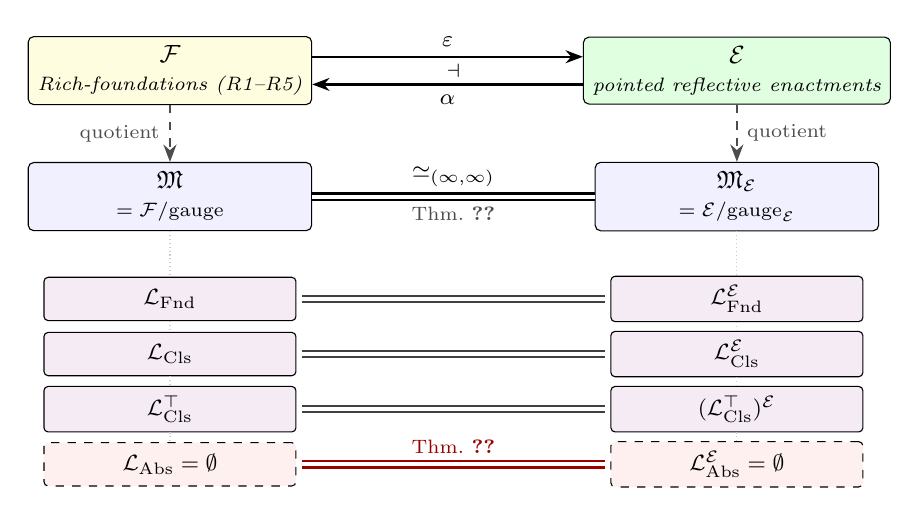
\begin{tikzpicture}[
  cat/.style={draw, rounded corners=2pt, minimum width=3.6cm, minimum height=0.85cm, align=center, font=\small},
  stack/.style={draw, rounded corners=2pt, minimum width=3.6cm, minimum height=0.85cm, align=center, font=\small, fill=blue!6},
  strat/.style={draw, rounded corners=1.5pt, minimum width=3.2cm, minimum height=0.55cm, align=center, font=\footnotesize, fill=violet!8},
  emptybox/.style={draw, dashed, rounded corners=1.5pt, minimum width=3.2cm, minimum height=0.55cm, align=center, font=\footnotesize, fill=red!6},
  func/.style={-{Stealth[length=2.2mm]}, thick},
  equiv/.style={thick, double, double distance=1.5pt},
  node distance=0.4cm
]
% Top row: 2-categories
\node[cat, fill=yellow!12] (F) at (-3.6,3.2) {$\cF$ \\[-1pt] \scriptsize\itshape Rich-foundations (R1--R5)};
\node[cat, fill=green!12] (E) at (3.6,3.2) {$\cE$ \\[-1pt] \scriptsize\itshape pointed reflective enactments};
\draw[func] ([yshift=5pt]F.east) -- node[midway, above, font=\footnotesize] {$\varepsilon$} ([yshift=5pt]E.west);
\draw[func] ([yshift=-5pt]E.west) -- node[midway, below, font=\footnotesize] {$\alpha$} ([yshift=-5pt]F.east);
\node[font=\scriptsize] at (0, 3.2) {$\dashv$};

% Middle row: moduli stacks
\node[stack] (M) at (-3.6, 1.6) {$\fM$ \\[-1pt] \scriptsize\itshape $= \cF / \mathrm{gauge}$};
\node[stack] (ME) at (3.6, 1.6) {$\fME$ \\[-1pt] \scriptsize\itshape $= \cE / \mathrm{gauge}_\cE$};
\draw[func, dashed, gray!60!black] (F) -- node[midway, left, font=\scriptsize, gray!60!black] {quotient} (M);
\draw[func, dashed, gray!60!black] (E) -- node[midway, right, font=\scriptsize, gray!60!black] {quotient} (ME);
\draw[equiv] (M.east) -- node[midway, above, font=\footnotesize] {$\simeq_{(\infty, \infty)}$} node[midway, below, font=\scriptsize, gray!60!black] {Thm.~\ref{thm:ac-oc-duality}} (ME.west);

% Bottom rows: strata correspondence
\node[strat] (L5F) at (-3.6, 0.3) {$\LFnd$};
\node[strat] (L5E) at (3.6, 0.3) {$\LFndE$};
\node[strat] (LCF) at (-3.6, -0.4) {$\LCls$};
\node[strat] (LCE) at (3.6, -0.4) {$\LClsE$};
\node[strat] (LMF) at (-3.6, -1.1) {$\LClsMax$};
\node[strat] (LME) at (3.6, -1.1) {$\LClsMaxE$};
\node[emptybox] (L6F) at (-3.6, -1.8) {$\LAbs = \emptyset$};
\node[emptybox] (L6E) at (3.6, -1.8) {$\LAbsE = \emptyset$};

\draw[equiv, gray!50!black, shorten >=2pt, shorten <=2pt] (L5F) -- (L5E);
\draw[equiv, gray!50!black, shorten >=2pt, shorten <=2pt] (LCF) -- (LCE);
\draw[equiv, gray!50!black, shorten >=2pt, shorten <=2pt] (LMF) -- (LME);
\draw[equiv, red!60!black, shorten >=2pt, shorten <=2pt] (L6F) -- node[midway, above, font=\scriptsize, red!60!black] {Thm.~\ref{thm:dual-afnt}} (L6E);

% Connect stacks to strata
\draw[gray!40, densely dotted] (M.south) -- (L5F.north);
\draw[gray!40, densely dotted] (ME.south) -- (L5E.north);
\draw[gray!40, densely dotted] (L5F.south) -- (LCF.north);
\draw[gray!40, densely dotted] (L5E.south) -- (LCE.north);
\draw[gray!40, densely dotted] (LCF.south) -- (LMF.north);
\draw[gray!40, densely dotted] (LCE.south) -- (LME.north);
\draw[gray!40, densely dotted] (LMF.south) -- (L6F.north);
\draw[gray!40, densely dotted] (LME.south) -- (L6E.north);

\end{tikzpicture}
\caption{AC/OC duality and the induced bijection of strata. At the $2$-category level (top row), the adjoint pair $\varepsilon \dashv \alpha$ (Definition~\ref{def:enactments}) relates the theory-centric $\cF$ to the enactment-centric $\cE$: $\varepsilon$ is the syntactic self-enactment section $F \mapsto (F, \Syn(F), \id, \id)$; $\alpha$ is the forgetful functor $(F, \cC, \iota, r) \mapsto F$. Passing to gauge-classes (middle row) yields an $(\infty, \infty)$-equivalence of classifying $2$-stacks $\fM \simeq \fME$ (Theorem~\ref{thm:ac-oc-duality}), via full faithfulness of $\varepsilon$ and essential surjectivity through the chosen reflector $r$. Under this equivalence the four strata correspond bijectively (bottom rows): $\LFnd \leftrightarrow \LFndE$, $\LCls \leftrightarrow \LClsE$, $\LClsMax \leftrightarrow \LClsMaxE$, and $\LAbs = \emptyset \leftrightarrow \LAbsE = \emptyset$ (Theorem~\ref{thm:dual-afnt}). The symmetry formalises the reconciliation of the object-centric and action-centric viewpoints on mathematical foundations: neither is primary; both describe the same classifying stack.}
\label{fig:ac-oc-duality}
\end{figure}

\subsection{\texorpdfstring{The $2$-Category of Rich-Enactments}{The 2-Category of Rich-Enactments}}

\begin{definition}[$2$-category of enactments $\cE$]\label{def:enactments}
The \emph{$2$-category of Rich-enactments} $\cE$ has:
\begin{itemize}
\item \textbf{Objects}: quadruples $(F, \cC, \iota, r)$, called \emph{pointed reflective enactments over $F$}, where $F \in \cF$, $\cC \in \mathbf{StrCat}_{S, n_F}$ (Definition~\ref{def:strcat}) is a $\kappa_1$-accessible $S$-model-category with an $F$-model structure, $\iota : \Syn(F) \to \cC$ is an $F$-preserving fully faithful $(\infty, n_F)$-functor onto a replete sub-$(\infty, n_F)$-category, and $r : \cC \to \Syn(F)$ is a \emph{chosen} left adjoint (reflector) to $\iota$ with unit $\eta_r : \id_\cC \Rightarrow \iota \circ r$ and counit $\varepsilon_r : r \circ \iota \Rightarrow \id_{\Syn(F)}$ satisfying the triangle identities in $\mathbf{StrCat}_{S, n_F}$. The reflector $r$ is part of the data; it is uniquely determined by $\iota$ up to unique invertible $2$-cell (Riehl--Verity~\cite{RiehlVerity2022} Prop.~2.1.11; Ad\'amek--Rosick\'y~\cite{AdamekRosicky1994} Thm.~1.26).
\item \textbf{$1$-morphisms} $(\phi, \Phi) : (F_1, \cC_1, \iota_1, r_1) \to (F_2, \cC_2, \iota_2, r_2)$: a pair consisting of a $1$-morphism $\phi : F_1 \to F_2$ in $\cF$ (faithful interpretation) and an $S$-preserving $(\infty, n)$-functor $\Phi : \cC_1 \to \cC_2$ equipped with an invertible $2$-cell $\Phi \circ \iota_1 \Rightarrow \iota_2 \circ \Syn(\phi)$;
\item \textbf{$2$-morphisms}: coherent natural transformations $(\phi, \Phi) \Rrightarrow (\phi', \Phi')$ compatible with the structure cells, i.e., pairs $(\tau, T)$ with $\tau : \phi \Rightarrow \phi'$ in $\cF$ and $T : \Phi \Rrightarrow \Phi'$ satisfying the evident pentagon with $\iota_1, \iota_2, \Syn(\tau)$.
\end{itemize}
There is a canonical forgetful $2$-functor and a canonical section:
\[
  \alpha : \cE \to \cF, \quad (F, \cC, \iota, r) \mapsto F; \qquad
  \varepsilon : \cF \to \cE, \quad F \mapsto \bigl(F,\, \Syn(F),\, \id_{\Syn(F)},\, \id_{\Syn(F)}\bigr).
\]
By construction $\alpha \circ \varepsilon = \id_\cF$ strictly. For readability I occasionally write $(F, \cC, \iota)$ for $(F, \cC, \iota, r)$ when the reflector is understood.
\end{definition}

\subsection{The Enactment Syntax--Semantics Lemma}

\begin{definition}[The class $\SSE$]\label{def:SSE}
Given $S \in \RS$, the class $\SSE \subseteq \Ob \cE$ of \emph{$S$-definable pointed enactments} is the closure of the base class
\[
  \SSEbase = \bigl\{ (F', \cM, \iota_\cM, r_\cM) : \cM \models S,\ F' \in \cF,\ \iota_\cM := \ev_\cM,\ r_\cM := (\ev_\cM)^L \bigr\},
\]
where $\ev_\cM : \Syn(F') \to \cM$ is the syntax-to-semantics evaluation of (R5b) and $(\ev_\cM)^L$ is its left adjoint (Lambek--Scott), under componentwise application of the operations of Definition~\ref{def:SS}: the $F$-component by Definition~\ref{def:SS}; the $\cC$-component via the forgetful $\mathbf{StrCat}_{S, n} \to (\infty, n)\text{-}\Cat$; the $(\iota, r)$-components by functoriality of adjunctions under $S$-preserving $(\infty, n)$-functors. The sub-class $\SSEglobal \subseteq \SSE$ is the corresponding closure of $\SSEbase$ using only those operations of Definition~\ref{def:SS} defining $\cS_S^{\mathrm{global}}$ (Kan extensions, Grothendieck constructions, derived functors).
\end{definition}

\begin{lemma}[Enactment syntax--semantics lemma]\label{lem:SS-membership-E}
Let $(F, \cC, \iota, r) \in \cE$ be a pointed reflective enactment such that the quadruple is formally $S$-definable, i.e., there exist formulas $\phi_F, \psi_\cC, \chi_\iota, \chi_r$ in some $F' \in \cF$ with $F' \hookrightarrow S$ specifying $F, \cC, \iota, r$ respectively, with the triangle identities and reflectiveness of $\iota$ provable in $F'$. Then $(F, \cC, \iota, r) \in \SSEglobal$.
\end{lemma}

\begin{proof}
By hypothesis, $F$ is formally $S$-definable via $\phi_F$; Lemma~\ref{lem:SS-membership} gives $F \in \cS_S^{\mathrm{global}}$. The model-category $\cC$ is specified by $\psi_\cC$ within $F'$; as an $S$-structured $(\infty, n)$-category the underlying $(\infty, n)$-category of $\cC$ lies in $\cS_S^{\mathrm{global}}$ by the same argument applied to the $\cS_S^{\mathrm{global}}$-closure of Definition~\ref{def:SS}. The pointing $\iota$ and the reflector $r$, specified by $\chi_\iota$ and $\chi_r$ in $F'$, are morphisms between $\cS_S^{\mathrm{global}}$-objects definable in $F' \hookrightarrow S$; by functoriality of adjunctions (the Lambek--Scott $\Syn \dashv \Mod$ extends to adjunctions in the syntactic $2$-category, which commutes with $S$-definable functorial operations), the adjoint pair $(\iota, r)$ with triangle identities belongs to the natural-transformation / Kan-extension closure of Definition~\ref{def:SS}. Assembled componentwise, $(F, \cC, \iota, r) \in \SSEglobal$.
\end{proof}

\subsection{AC/OC Morita Duality}

\begin{theorem}[AC/OC Morita Duality --- formal-organizational form]\label{thm:ac-oc-duality}

The adjoint pair $\varepsilon \dashv \alpha$ of Definition~\ref{def:enactments} induces an $(\infty, \infty)$-equivalence of classifying $2$-stacks
\[
  \fM \;\simeq_{(\infty, \infty)}\; \fM_\cE, \qquad \fM_\cE := \cE / \mathrm{gauge}_\cE,
\]
where the left-hand moduli stack is the classifying $2$-stack of $\cF$ from Convention~\ref{conv:notation} and $\fM_\cE$ is the corresponding classifying $2$-stack of $\cE$. Concretely:
\begin{enumerate}[label=(\alph*)]
\item $\varepsilon : \cF \to \cE$ is fully faithful;
\item the unit $\id_\cF \Rightarrow \alpha \circ \varepsilon$ is an equality; the counit $\varepsilon \circ \alpha \Rightarrow \id_\cE$ is a gauge-equivalence, i.e., an equivalence after passing to $\fM_\cE$;
\item the strata $\LFnd, \LCls, \LClsMax, \LAbs$ of $\fM$ correspond bijectively to strata $\LFnd^\cE, \LCls^\cE, (\LClsMax)^\cE, \LAbs^\cE$ of $\fM_\cE$ via the induced equivalence, preserving the meta-operations $\mathrm{Cls}$ and $\mathrm{Gen}$.
\end{enumerate}
\end{theorem}

\begin{proof}
\emph{(a) Full faithfulness of $\varepsilon$.} Let $F_1, F_2 \in \cF$. Unpacking Definition~\ref{def:enactments}, a $1$-morphism $\varepsilon(F_1) \to \varepsilon(F_2)$ is a pair $(\phi, \Phi)$ with $\phi : F_1 \to F_2$ in $\cF$ and $\Phi : \Syn(F_1) \to \Syn(F_2)$ an $S$-preserving $(\infty, n)$-functor equipped with an invertible $2$-cell $\Phi \Rightarrow \Syn(\phi)$. The $2$-functoriality of $\Syn : \cF \to \mathbf{StrCat}_{S, n}$, guaranteed by Lambek--Scott for $n = 1$ (Lurie HTT~\cite{LurieHTT} \S 5.1) and for general $n$ by the Kapulkin--Lumsdaine~\cite{KapulkinLumsdaine2021} assembly of $\Syn \dashv \Mod$ as a $2$-functor on syntactic $(\infty, n)$-categories, ensures that every $S$-preserving $(\infty, n)$-functor $\Syn(F_1) \to \Syn(F_2)$ arises, up to an invertible $2$-cell, from $\Syn(\phi)$ for a unique $\phi : F_1 \to F_2$. Hence the forgetful map of hom-$2$-categories
\[
  \Hom_{\cE}(\varepsilon F_1, \varepsilon F_2) \longrightarrow \Hom_{\cF}(F_1, F_2), \qquad (\phi, \Phi) \mapsto \phi,
\]
is an $(\infty, 2)$-equivalence. This establishes full faithfulness of $\varepsilon$ at every hom-$2$-category.

\emph{(b) Essential surjectivity at gauge level.} Let $(F, \cC, \iota, r) \in \cE$. The reflector $r$ is part of the object data and, being left adjoint to a fully faithful functor, has invertible counit $\varepsilon_r : r \circ \iota \Rightarrow \id_{\Syn(F)}$ (standard: Riehl--Verity~\cite{RiehlVerity2022} Prop.~2.1.11). Define an $\cE$-morphism $(\id_F, r) : (F, \cC, \iota, r) \to \varepsilon(F) = (F, \Syn(F), \id, \id)$ using $r$ as the underlying functor $\cC \to \Syn(F)$; its structure cell $r \circ \iota \Rightarrow \id \circ \Syn(\id_F) = \id_{\Syn(F)}$ is precisely $\varepsilon_r$. The reverse $(\id_F, \iota) : \varepsilon(F) \to (F, \cC, \iota, r)$ is the pointing. The composite
\[
  (\id_F, \iota) \circ (\id_F, r) = (\id_F, \iota \circ r)
\]
satisfies $\iota \circ r \simeq \id_\cC$ via the unit $\eta_r$ of the adjunction, hence is gauge-equivalent to $\id$ in $\cE$; conversely, $(\id_F, r) \circ (\id_F, \iota) = (\id_F, r \circ \iota) \simeq (\id_F, \id_{\Syn(F)}) = \id_{\varepsilon(F)}$ via $\varepsilon_r$. This yields a canonical gauge-equivalence
\[
  (F, \cC, \iota, r) \;\simeq_{\mathrm{gauge}_\cE}\; \varepsilon(F) \quad\text{in } \fM_\cE.
\]
Uniqueness of $r$ up to unique invertible $2$-cell given $\iota$ makes this equivalence natural in the object. Hence $\varepsilon$ is essentially surjective after passing to gauge-classes.

Combined with (a), the pair $(\varepsilon, \alpha)$ induces an equivalence $\fM \simeq \fM_\cE$ at the $(\infty, 2)$-level.

\emph{Lift to $(\infty, \infty)$.} The argument above is parametric in $n \in \mathbb{N} \cup \{\infty\}$: it uses only (R5b), the $2$-functoriality of $\Syn$ over $n$, and the uniqueness of reflectors at $(\infty, n)$. The first is (R5b); the second is Kapulkin--Lumsdaine~\cite{KapulkinLumsdaine2021} combined with Barwick--Schommer-Pries~\cite{BarwickSchommerPries2021}; the third is Ad\'amek--Rosick\'y~\cite{AdamekRosicky1994} Thm.~1.26 applied slice-wise via Lurie HTT~\cite{LurieHTT} \S 5.4 ($\lambda$-filtered-colimit preservation by accessible adjunctions). Stabilization of the equivalence at $n = \infty$ follows from Theorem~\ref{thm:bergner-lurie-stab}.

\emph{(c) Stratum correspondence.} The classification meta-operation $\mathrm{Cls}$ on $\fM$ sends $F \in \LFnd$ to its class of classifiable sub-stacks. Under the equivalence $\fM \simeq \fM_\cE$, the enactment $\varepsilon(F) = (F, \Syn(F), \id, \id)$ inherits the classification structure via $\iota = \id$, i.e., $\mathrm{Cls}^\cE(\varepsilon F)$ coincides with $\varepsilon$ applied to $\mathrm{Cls}(F)$. Analogously for $\mathrm{Gen}$. The strata $\LClsE \supsetneq \LClsMaxE \supseteq \LAbsE$ on $\fM_\cE$ are defined by the $\cE$-analogues of Definition~\ref{def:hierarchy}: a gauge-class $[(F, \cC, \iota, r)] \in \LClsE$ iff $[F] \in \LCls$; similarly for the finer strata. Under this translation, the equivalence of (a)--(b) restricts to a bijection of strata.
\end{proof}

\begin{corollary}[Conservativity; consistency strength]\label{cor:ac-oc-conservativity}
The extension of the MSFS framework by $\cE$ and the structure maps $(\alpha, \varepsilon)$ is a conservative extension of the $\cF$-based framework. In particular,
\[
  \Con(\cF \cup \cE) \;=\; \Con(\cF) \;=\; \Con(\ZFC + 2\text{-inacc}).
\]
\end{corollary}

\begin{proof}
By Theorem~\ref{thm:ac-oc-duality}, every statement about $\fM_\cE$ translates to an equivalent statement about $\fM$ via the equivalence. No new axioms are introduced; by, $\cE$ is $\mathbf{U}_2$-small and is constructed inside $\ZFC + 2\text{-inacc}$ from $\cF$ and $\mathbf{StrCat}_{S, n}$ (Definition~\ref{def:strcat}) using only Lambek--Scott adjunctions guaranteed by (R5b) and reflectors given as object data (Definition~\ref{def:enactments}).
\end{proof}

The equivalence of Theorem~\ref{thm:ac-oc-duality} transfers the $\LAbs$ conditions of \S\ref{sec:conditions} to the enactment side. Informally, an \emph{enactment-absolute} triple $(F, \cC, \iota)$ is one whose enactment-side description simultaneously admits formal specification, admits no non-trivial coordination with other enactments in the $S$-definable class, and is maximally receptive (every other enactment factors through it).

\begin{definition}[$\LAbsE$ conditions]\label{def:level6-cE}
Given $S \in \RS$ and $n \in \mathbb{N} \cup \{\infty\}$, a pointed reflective enactment $(F, \cC, \iota, r) \in \cE$ is \textbf{enactment-absolute} if it satisfies the triple:
\begin{itemize}
\item[$(\tilde{F}_S)$] \emph{Enactment-definability}: the quadruple $(F, \cC, \iota, r)$ is formally $S$-definable in the sense of Lemma~\ref{lem:SS-membership-E}, i.e., specified by formulas $(\phi_F, \psi_\cC, \chi_\iota, \chi_r)$ in some $F' \in \cF$ with $F' \hookrightarrow S$ (this refines $(F_S)$ by additionally specifying the model-category presentation, the pointing, and the reflector).
\item[$(\tilde{\Pi}_{4, S, n})$] \emph{Non-coordination}: there is no $1$-morphism $(\phi, \Phi) : (F, \cC, \iota, r) \to (F', \cC', \iota', r')$ in $\cE$ with target quadruple in $\SSE$ (Definition~\ref{def:SSE}) such that $\Phi$ is an $(\infty, n)$-equivalence onto its image.
\item[$(\tilde{\Pi}_{3\text{-max}, S, n})$] \emph{Maximal receptivity}: for every enactment $(F', \cC', \iota', r') \in \cE$ there exists a $1$-morphism $(\phi, \Phi) : (F', \cC', \iota', r') \to (F, \cC, \iota, r)$ realizing a Morita reduction at the $(\infty, n)$-level.
\end{itemize}
The \emph{$\LAbsE$ stratum} is the class of $\mathrm{gauge}_\cE$-equivalence classes in $\fM_\cE$ with an enactment-absolute representative.
\end{definition}

\subsection{Dual Boundary Lemma}

\begin{theorem}[Dual Boundary Lemma; Dual-AFN-T $(\alpha)$-part]\label{thm:dual-afnt}
For every Rich-metatheory $S \in \RS$ and every categorical level $n \in \mathbb{N} \cup \{\infty\}$, no pointed reflective enactment $(F, \cC, \iota, r) \in \cE$ satisfies the $\LAbsE$ triple $(\tilde{F}_S) \wedge (\tilde{\Pi}_{4, S, n}) \wedge (\tilde{\Pi}_{3\text{-max}, S, n})$. Already the sub-pair $(\tilde{F}_S) \wedge (\tilde{\Pi}_{4, S, n})$ is structurally self-contradictory.
\end{theorem}

\begin{proof}
Suppose $(F, \cC, \iota, r) \in \cE$ satisfies $(\tilde{F}_S) \wedge (\tilde{\Pi}_{4, S, n})$. By Lemma~\ref{lem:SS-membership-E}, $(F, \cC, \iota, r) \in \SSEglobal \subseteq \SSE$. The identity $1$-morphism $(\id_F, \id_\cC)$ has $\Phi = \id_\cC$ an $(\infty, n)$-equivalence onto its image, with target in $\SSE$. This coordination is forbidden by $(\tilde{\Pi}_{4, S, n})$. Contradiction. Hence $\LAbsE = \emptyset$.
\end{proof}

\begin{corollary}[$\LAbsE$ emptiness]\label{cor:level6-empty-cE}
$\LAbsE = \emptyset$.
\end{corollary}

\begin{theorem}[Dual five-axis absoluteness]\label{thm:dual-five-axis}
Theorems~\ref{thm:horizontal}--\ref{thm:completeness} transfers to $\LAbs^\cE$: the emptiness of $\LAbs^\cE$ is absolute along the five structural axes
\begin{center}
\emph{horizontal} (over $\RS$), \quad \emph{vertical} (over $n$), \quad \emph{meta-vertical}, \quad \emph{lateral}, \quad \emph{completeness} (within Lawvere-scope).
\end{center}
In particular, the three standard bypass paths (Theorems~\ref{thm:universe}, \ref{thm:reflective}, \ref{thm:slice-locality}) foreclose their $\cE$-analogues.
\end{theorem}

\begin{proof}
Each axis transfers via Theorem~\ref{thm:ac-oc-duality} componentwise: the five mechanisms of Theorems~\ref{thm:horizontal}--\ref{thm:completeness} act parametrically on the $F$-component or naturally on the $\cC$-component of $(F, \cC, \iota, r)$, and the pair $(\alpha, \varepsilon)$ preserves them. Lawvere-scope $\mathrm{LS}(\cE)$ is defined as enactments with $F \in \mathrm{LS}(\cF)$ and $\cC$ closed symmetric monoidal (Cartesian-closed or $*$-autonomous, covering linear logic and quantum-categorical enactments); Yanofsky's~\cite{Yanofsky2003} generalized diagonal applies in $\cC$ and transports to $\Syn(F)$ via $\iota \dashv r$. The three bypass paths transfer analogously via the componentwise action of $(\alpha, \varepsilon)$.
\end{proof}

\section{Placement in the No-Go Series}\label{sec:series}

AFN-T occupies a position in the structural series of foundational no-go theorems. All such results instantiate a single categorical schema: \emph{a system sufficiently expressive to formulate a candidate maximal object is unable to contain that object without contradiction}, realized through a self-referential embedding that turns the purported maximal object into an element of the very class it was supposed to transcend. Each specializes the schema through a distinct maximality aspect and diagonal step:

\begin{center}
\begin{tabular}{@{}l l p{3.2cm} p{5.7cm}@{}}
\toprule
Theorem & Year & Maximality aspect & Diagonal step \\ \midrule
Cantor~\cite{Cantor1891} & 1891 & cardinal & $x \notin f(x)$ for $f : X \to \cP(X)$ \\
Russell~\cite{Russell1903} & 1901 & comprehension & $R = \{x : x \notin x\}$, $R \in R \iff R \notin R$ \\
G\"odel (I, II)~\cite{Godel1931} & 1931 & completeness / consistency & $G = $ ``$G$ is not provable'' \\
Tarski~\cite{Tarski1936} & 1936 & semantic truth & ``this sentence is not true'' \\
Lawvere FP~\cite{Lawvere1969} & 1969 & categorical fixed-point & cartesian-closed + weakly surjective $\Rightarrow$ every $f$ has a fixed point \\
Ernst~\cite{Ernst2015} & 2015 & unlimited category theory & Lawvere diagonal at $n = 1$ under Feferman (R1)--(R3) \\
AFN-T & --- & foundational (definable + non-reducible + generative) & syntax--semantics bridge: $(F_S) \Rightarrow X \in \cS_S^{\mathrm{global}}$ via Lemma~\ref{lem:SS-membership}, contradicting $(\Pi_4)$ by $\id_X$ (Theorem~\ref{thm:afnt-alpha}) \\
Dual-AFN-T & --- & enactment-absolute (definable + non-coordination + receptive) & identity enactment $(\id_F, \id_\cC)$ with target in $\SSE$ (Lemma~\ref{lem:SS-membership-E}) contradicts $(\tilde{\Pi}_4)$ (Theorem~\ref{thm:dual-afnt}); equivalently via $\alpha$ + AFN-T \\
\bottomrule
\end{tabular}
\end{center}

\subsection{Subsumption}

\begin{theorem}[Subsumption via specialization (framework-level)]\label{thm:subsumption}
For each classical no-go theorem $T$ below, there exists a triple $(S_T, n_T, X_T)$ with $S_T \in \RS$, $n_T \in \mathbb{N} \cup \{\infty\}$, and $X_T$ the purported maximal object of $T$, such that (i) $X_T \models (F_{S_T})$; (ii) $X_T$ under the hypothesis of $T$ would satisfy $(\Pi_{4, S_T, n_T})$; (iii) Theorem~\ref{thm:afnt-alpha} applied at $(S_T, n_T)$ yields a structural contradiction with the existence of $X_T$ as $\LAbs$-candidate. The theorem provides the \emph{framework} in which each classical no-go inhabits; the row-specific diagonals (Cantor's $|X|<|\cP(X)|$, Russell's $R \in R \leftrightarrow R \notin R$, etc.)\ are independent classical proofs that refine the abstract $\id_{X_T}$-template into the specific witness used by $T$, and are not derived from AFN-T~$\alpha$ alone.
\begin{center}\small
\begin{tabular}{@{}l@{\ \ }l@{\ \ }l@{\ \ }l@{\ \ }l@{}}
\toprule
$T$ & $S_T$ & $X_T$ & $n_T$ & $(F_{S_T})$-witness \\ \midrule
Cantor~\cite{Cantor1891} & $\ZFC$ & $\cP : \mathbf{Set} \to \mathbf{Set}$ as universal & $1$ & $\phi_{\cP}(X, Y) \equiv Y = \{Z : Z \subseteq X\}$ \\
Russell~\cite{Russell1903} & Na\"ive ST & $R := \{x : x \notin x\}$ & $1$ & $\phi_R(x) \equiv x \notin x$ \\
G\"odel I~\cite{Godel1931} & $\mathsf{PA}$ & $G$ (unprovable sentence) & $1$ & $\phi_G \equiv \neg \mathrm{Prov}(\ulcorner G \urcorner)$ \\
G\"odel II~\cite{Godel1931} & $\mathsf{PA}$ & $\mathrm{Con}(\mathsf{PA})$ as $\mathsf{PA}$-provable & $1$ & $\phi_{\mathrm{Con}}$ via $\mathrm{Prov}$-predicate \\
Tarski~\cite{Tarski1936} & $\mathsf{Th}(\mathbb{N})$ & $T \subseteq \mathsf{Formulas}$ (truth pred.) & $1$ & $T(\phi) \equiv \phi$ for each $\phi$ \\
Lawvere FP~\cite{Lawvere1969} & CCC ext.\ of $\ZFC$ & weakly surj.\ $X$ with $f: X \to X^X$ & $1$ & $\phi_X$ in CCC-syntax \\
Ernst~\cite{Ernst2015} & Feferman's (R1)--(R3) & UCT object & $1$ & Feferman unlimited-axiom schema \\
\bottomrule
\end{tabular}
\end{center}
In each row, AFN-T at $(S_T, n_T)$ yields $\LAbs(S_T, n_T) = \emptyset$ at the row's maximality aspect; the classical diagonal of $T$ is the specific witness refinement establishing $T$ within the framework.
\end{theorem}

\begin{proof}
Each row's $X_T$ is $S_T$-definable by the listed formula (i), so $X_T \in \cS_{S_T}^{\mathrm{global}}$ by Lemma~\ref{lem:SS-membership}. $\id_{X_T} : X_T \to X_T$ violates $(\Pi_{4, S_T, n_T})$ per Theorem~\ref{thm:afnt-alpha}, so $X_T \notin \LAbs$. The row-specific diagonal reconstructs: Cantor by $|X| < |\cP(X)|$ refining $\id_{\cP}$; Russell by $R \in R \leftrightarrow R \notin R$ refining $\id_R$; G\"odel by $G$-sentence $\leftrightarrow \neg\mathrm{Prov}(\ulcorner G \urcorner)$; Tarski's liar; Lawvere's fixed-point formula $f(x_0) = x_0$ via $\lambda x. f(x)(x)$; Ernst by Feferman unlimited-axiom schema. Each refinement specializes the universal $\id_{X_T}$ template of Theorem~\ref{thm:afnt-alpha} to the row-specific formal witness.
\end{proof}

\section{Consequences and Open Questions}\label{sec:consequences}

\subsection{Consequences for Foundational Programmes}

AFN-T imposes a uniform structural bound on every current foundational programme: each inhabits $\LFnd$, or $\LCls$ (possibly with membership in the maximal sub-class $\LClsMax \subseteq \LCls$), with $\LAbs$ empty. Specifically:
\begin{itemize}\setlength{\itemsep}{1pt}
\item \textbf{Univalent Foundations} (Voevodsky~\cite{VoevodskyFoundations2010}; HoTT Book~\cite{HoTTBook2013}) is a $\LCls$ partial meta-framework (Theorem~\ref{thm:meta-mult}) classifying $\HoTT$-extensions; it cannot be elevated to $\LAbs$.
\item \textbf{Higher topos theory} (Lurie~\cite{LurieHTT}) and \textbf{cohesive framework} (Schreiber~\cite{Schreiber2013}) occupy Levels 5 and 5+ respectively.
\item \textbf{Condensed mathematics} (Clausen--Scholze~\cite{ClausenScholze2019}), \textbf{perfectoid geometry}, and \textbf{$\infty$-cosmoi} (Riehl--Verity) are bounded similarly; no $\LAbs$ escalation is possible.
\item \textbf{Proof assistants} (Coq, Lean, Agda) implement $\LFnd$ foundations ($\CIC$, $\CIC + \mathrm{Univalence}$, $\MLTT$); the plurality of such systems is the plurality of $\LFnd$.
\item \textbf{Categorical logic}: classification of foundational systems by $(\infty, n)$-categories and their meta-structures has an upper bound at $\LCls$, aligning with Barwick--Schommer-Pries~\cite{BarwickSchommerPries2021} unicity.
\end{itemize}

\paragraph{Diagnostic: which $\LAbs$ condition fails for specific candidates?} For each well-known candidate sometimes informally described as ``absolute'', the precise failure mode within AFN-T's formal framework can be identified.
\begin{itemize}\setlength{\itemsep}{1pt}
\item \emph{Univalent Foundations (UF)}: passes $(F_S)$ (formally definable as HoTT + univalence axiom schema), passes $(\Pi_{4, S, n})$ conditionally (not Morita-reducible to $\ZFC$-internal structures, in the forward direction), but \emph{fails $(\Pi_{3\text{-max}, S, n})$}: UF does not classify Rich-foundations outside the HoTT-adjacent family (e.g., it does not classify ZFC-specific cardinal arithmetic or noncommutative-geometric spectral triples by Morita reduction). Hence UF $\in \LCls \setminus \LClsMax$.
\item \emph{Higher topos theory (Lurie)}: passes $(F_S)$, fails $(\Pi_{3\text{-max}})$ for essentially the same reason: classifies categorical structures of HoTT-compatible shape but does not subsume foundations outside this class.
\item \emph{Cohesive framework (Schreiber)}: passes $(F_S)$, fails $(\Pi_{3\text{-max}})$; additionally the cohesion axioms specialize to geometric contexts, further restricting the classification image.
\item \emph{$\infty$-cosmoi (Riehl--Verity)}: passes $(F_S)$ (axiomatized in $\ZFC + 2\text{-inacc}$), fails $(\Pi_{3\text{-max}})$; they classify $(\infty, 1)$-categorical structures, not the full $\fM$.
\item \emph{Any hypothetical candidate $X$ satisfying $(F_S) \wedge (\Pi_{3\text{-max}})$}: by Theorem~\ref{thm:afnt-alpha}, $X$ then fails $(\Pi_{4, S, n})$: if $X$ were both formally definable (via $(F_S)$) and maximally generative (via $(\Pi_{3\text{-max}})$), then by Lemma~\ref{lem:SS-membership} $X \in \cS_S^{\mathrm{global}}$ and $\id_X$ would realize a Morita reduction to an $\cS_S$-target, contradicting $(\Pi_{4, S, n})$.
\end{itemize}
Thus the three conditions cannot all simultaneously hold: current candidates fail $(\Pi_{3\text{-max}})$; any hypothetical stronger candidate satisfying $(F_S) \wedge (\Pi_{3\text{-max}})$ would fail $(\Pi_{4, S, n})$. The diagnostic identifies the precise obstruction in each case rather than merely asserting impossibility.

\subsection{Open Questions}

\paragraph{(Q1) Existence of a maximal meta-framework.} Theorem~\ref{thm:meta-cat} asserts categoricity of $\Meta_{\mathrm{Cls}}^{\top}$ conditional on its non-emptiness. Is there a concrete $\mathbf{F} \in \Meta_{\mathrm{Cls}}^{\top}$ constructible in $\ZFC + 2\text{-inacc}$? A positive answer would identify the canonical $\LCls$ meta-framework up to $(\infty, \infty)$-equivalence. The construction of such a witness lies outside the scope of this preprint; a candidate framework is the subject of separate ongoing work. Non-emptiness of $\Meta_{\mathrm{Cls}}^{\top}$ is an existential question with \emph{four independent structural obstacles}, corresponding to the four maximality conditions: (Max-1) requires a classifier with classification essentially surjective onto the entire $\fM$; (Max-2) requires a transitive $\mathrm{Aut}_2$-action on gauge classes; (Max-3) requires $\omega$-depth predicative filtration satisfying the comprehension-schema condition; and (Max-4) requires a canonical intensional completion $\II_{\mathbf{F}} : \mathbf{F}^{\mathrm{op}} \to \Sint$ satisfying (I-1)--(I-4). Of these, (Max-4) presents a distinct existential obstacle separate from (Max-1)--(Max-3): the construction of $\II_\mathbf{F}$ as a canonical completion (not merely existing, but canonically determined by the classifier structure) is non-trivial even granting the first three conditions. Resolution of Q1 accordingly reduces to the independent construction of each of the four structural data on a common underlying classifier, not to a single sufficient condition.

\paragraph{(Q2) Completeness of the meta-framework list.} How complete is the list $\{\mathbf{F}_{\mathrm{univalent}},\allowbreak \mathbf{F}_{\mathrm{cosmoi}},\allowbreak \mathbf{F}_{\mathrm{cohesive}},\allowbreak \mathbf{F}_{\mathrm{HA}},\allowbreak \mathbf{F}_{\mathrm{synthetic}}\}$ of currently identified $\LCls$ meta-structures ($\mathbf{F}_{\mathrm{HA}}$ denotes Lurie's Higher Algebra programme~\cite{LurieHA})? Are there further natural meta-frameworks?

\paragraph{(Q3) Exhaustiveness of bypass paths.} Theorems~\ref{thm:universe}, \ref{thm:reflective}, \ref{thm:I-existence}, \ref{thm:slice-locality} close three standard bypass paths, and Appendix~\ref{app:paraconsistent} treats the paraconsistent case. Candidates for additional independent paths include modal or temporal logic extensions, substructural logics without exponential $!$, realizability and constructive-only foundations, and foundations grounded in non-classical computability models. Each of these appears to reduce to one of the closed paths within R-S; a formal exhaustiveness theorem is not given here and remains open.

\paragraph{(Q4) Consistency-strength minimality.} The proof uses $\ZFC + 2\text{-inacc}$ (Convention~\ref{conv:zfc-inacc}). Can a weaker consistency strength suffice for the full theorem, or does the meta-classification stabilization (Theorem~\ref{thm:meta-stab}) genuinely require the second inaccessible?

\paragraph{(Q5) Sub-stack of weak Rich-metatheories.} Do bounded-arithmetic theories ($\mathsf{I\Delta_0}$, $\mathsf{S}_2^i$) satisfying (R2)--(R5) and a restricted (R1) form a separate stratum $\LFnd^{\mathrm{weak}} \subset \LFnd$, or are they Morita-dense in $\LFnd$ via reverse mathematics~\cite{Simpson2009}?

\appendix

\section{Categorical Preliminaries}\label{app:categorical}

I collect here the categorical tools and standard theorems invoked in the proofs above.

\subsection{\texorpdfstring{$2$-Categories}{2-Categories}}

A \textbf{$2$-category} $\cC$ consists of:
\begin{itemize}
\item A class of objects $\Ob(\cC)$.
\item For each pair $A, B \in \Ob(\cC)$, a small category $\Hom_\cC(A, B)$ of $1$-morphisms and $2$-morphisms.
\item Composition functors and identity $1$-morphisms satisfying standard $2$-categorical coherence.
\end{itemize}

A $2$-category is \textbf{locally small} if each $\Hom_\cC(A, B)$ is a small category. All $2$-categories in this paper are locally small unless stated otherwise.

Reference: Kelly~\cite{Kelly1982} for enriched and $2$-categorical foundations; B\'enabou~\cite{Benabou1967} for bicategories.

\subsection{\texorpdfstring{$(\infty, n)$-Categories}{(infinity,n)-Categories}}

An $(\infty, n)$-category is a generalization of category theory where:
\begin{itemize}
\item Morphisms have $k$-morphisms for $k \leq n$.
\item $k$-morphisms for $k > n$ are all invertible (equivalences).
\end{itemize}

Models include: quasi-categories, Segal $n$-categories, complete Segal spaces, $\Theta_n$-spaces. Equivalence of these models is established by Ara--Maltsiniotis~\cite{AraMaltsiniotis2017}.

The $(\infty, n)$-hierarchy stabilizes at $n = \infty$: the canonical inclusion $(\infty, \infty)\text{-}\Cat \hookrightarrow (\infty, \infty + 1)\text{-}\Cat$ is an equivalence (Barwick--Schommer-Pries~\cite{BarwickSchommerPries2021}, applied iteratively over the Bergner--Rezk~\cite{BergnerRezk2013} comparison of models).

Reference: Lurie HTT~\cite{LurieHTT} for $(\infty, 1)$-categories; Riehl--Verity~\cite{RiehlVerity2022} for synthetic $(\infty, 1)$-category theory.

\subsection{Accessible Functors}

A functor $F : \cC \to \cD$ between locally small categories is \textbf{$\lambda$-accessible} (for a regular cardinal $\lambda$) if $F$ preserves $\lambda$-filtered colimits.

A category $\cC$ is \textbf{locally $\lambda$-presentable} if it is cocomplete and has a small dense subcategory of $\lambda$-presentable objects.

Reference: Ad\'amek--Rosick\'y~\cite{AdamekRosicky1994} for accessibility theory.

\begin{lemma}[Lair--Makkai--Par\'e representation, informal]\label{lem:lair}
Every accessible category is $2$-categorically equivalent to the $2$-category of models of a small sketch; equivalently, to the $2$-category of models of an accessible $2$-theory.
\end{lemma}

Reference: Lair~\cite{Lair1981} (original French version for $1$-categorical sketches); Makkai--Par\'e~\cite{MakkaiPare1989} Chapter 3 (systematic development, including the $2$-categorical sketch/theory correspondence); Ad\'amek--Rosick\'y~\cite{AdamekRosicky1994} Chapter 2 (accessibility-theoretic treatment).

\subsection{Display Map Categories}

\begin{definition}[Display map category, $1$-categorical version]\label{def:display-1cat}
A \textbf{display map category} is a pair $(\cC, \cD)$ where $\cC$ is a category with pullbacks and $\cD \subseteq \Mor(\cC)$ is a class of morphisms stable under pullback and containing isomorphisms.
\end{definition}

Jacobs~\cite{Jacobs1999} establishes that display map categories provide categorical semantics for intensional type theories, with display morphisms corresponding to dependent type families.

Gambino--Garner~\cite{GambinoGarner2008} extends this to the $2$-categorical setting, yielding Definitions~\ref{def:display-class} and~\ref{def:display-2-cat}.

\subsection{Bicategory of Fractions}

\begin{lemma}[Pronk's bicategory of fractions]\label{lem:pronk}
Given a $2$-category $\cC$ and a class $\mathcal{W}$ of $1$-morphisms satisfying the Bousfield--Pronk calculus-of-fractions conditions (BF1)--(BF5), the $2$-localization $\cC[\mathcal{W}^{-1}]$ exists as a bicategory of fractions.
\end{lemma}

Reference: Pronk~\cite{Pronk1996}.

The conditions (BF1)--(BF5) are:
\begin{itemize}
\item[\textbf{(BF1)}] Contains identities.
\item[\textbf{(BF2)}] Closed under composition.
\item[\textbf{(BF3)}] $2$-pullback stable.
\item[\textbf{(BF4)}] $2$-right-filtered (any morphism can be extended).
\item[\textbf{(BF5)}] $\mathcal{W}$-saturation: contains all $2$-equivalences.
\end{itemize}

\subsection{Lawvere Fixed-Point Theorem}

\begin{lemma}[Lawvere fixed-point, $2$-categorical]\label{lem:lawvere-2}
In a $2$-cartesian closed category $\cC$ with a weakly point-surjective $1$-morphism $e : A \to Y^A$, every $f : Y \to Y$ has a fixed point: there exists $y_0 : 1 \to Y$ with $f \circ y_0 = y_0$ up to coherent $2$-equivalence.
\end{lemma}

Reference: Lawvere~\cite{Lawvere1969}; Yanofsky~\cite{Yanofsky2003} for $2$-categorical formulation.

\begin{lemma}[Lawvere fixed-point, $(\infty, \infty)$-categorical]\label{lem:lawvere-inf}
In an $(\infty, \infty)$-cartesian closed category $\cC$ with a coherently surjective Yoneda embedding $y : \cC \hookrightarrow 2\text{-}\mathrm{PSh}(\cC)$, every $f : Y \to Y$ has an $(\infty, \infty)$-coherent fixed point.
\end{lemma}

This is obtained by extending Lemma~\ref{lem:lawvere-2} through the $\Theta_n$-space model of Rezk~\cite{Rezk2010}, passed to the limit $n \to \infty$ via the unicity theorem of Barwick--Schommer-Pries~\cite{BarwickSchommerPries2021}. The $(\infty, \infty)$-coherent fixed point is the canonical limit of the compatible family of fixed points constructed at each finite $n$.

\subsection{Whitehead-Type Criterion}

\begin{lemma}[Whitehead-type equivalence criterion]\label{lem:whitehead}
Let $\Phi : \cC_1 \to \cC_2$ be an $(\infty, \infty)$-functor between accessible $(\infty, \infty)$-categories. Then $\Phi$ is an $(\infty, \infty)$-equivalence if and only if its truncations $\tau_{\leq n}(\Phi) : \tau_{\leq n}(\cC_1) \to \tau_{\leq n}(\cC_2)$ are $(\infty, n)$-equivalences for every $n \in \mathbb{N}$.
\end{lemma}

Reference: Lurie HTT~\cite{LurieHTT} \S 6.5.4 (``Whitehead's Theorem'' for $(\infty, 1)$-topoi) and \S 5.5.6 (truncated objects in $(\infty, 1)$-categories); Barwick--Schommer-Pries~\cite{BarwickSchommerPries2021} for the $(\infty, n)$-extension.

\subsection{Bergner--Lurie Stabilization}

\begin{theorem}[$(\infty, \infty)$-stabilization]\label{thm:bergner-lurie-stab}
The inclusion $(\infty, \infty)\text{-}\Cat \hookrightarrow (\infty, \infty + 1)\text{-}\Cat$ is an equivalence of $(\infty, \infty)$-categories.
\end{theorem}

Reference: Barwick--Schommer-Pries~\cite{BarwickSchommerPries2021} (unicity of the theory of higher categories); Bergner--Rezk~\cite{BergnerRezk2013} (comparison of models); Ara--Maltsiniotis~\cite{AraMaltsiniotis2017} (globular/cubical comparison).

\section{Paraconsistent Extension}\label{app:paraconsistent}

AFN-T as stated (Theorem~\ref{thm:afnt-alpha}) applies to classical Rich-metatheories. This appendix extends the result to paraconsistent Rich-metatheories \emph{with extractable classical kernel} --- the class of paraconsistent logics in which every theorem admits a classical-inference witness. The extension does \emph{not} cover strongly-dialetheic theories (see below).

\subsection{Paraconsistent R-S}

\begin{definition}[Paraconsistent R-S with extractable classical kernel]\label{def:paraconsistent-rs}
A theory $S'$ is a \textbf{paraconsistent Rich-metatheory with extractable classical kernel} if it satisfies the classical conditions (R1')--(R5') analogous to (R1)--(R5), together with:
\begin{itemize}
\item \textbf{(Explosion-min)}: $\bot \not\vdash \phi$ for every formula $\phi$ (contradictions do not entail everything).
\item \textbf{(Strong-neg)}: there exists a negation $\sim$ such that $(p \wedge \sim p) \vdash_\sim \bot$ (a specific contradiction principle, though not full explosion).
\item \textbf{(Classical-kernel extractability)}: the largest fragment $S'^* \subseteq S'$ closed under classical inference rules is itself consistent, non-empty, and a Rich-metatheory in $\RS$. Equivalently: every theorem of $S'$ of foundational significance (in particular, the defining formula of any $\LAbs$ candidate) admits a witness derivable purely by classical inference from $S'$'s classical-only axioms.
\end{itemize}
\end{definition}

\subsection{Paraconsistent AFN-T}

\begin{theorem}[Paraconsistent AFN-T]\label{thm:paraconsistent-afnt}
If $S'$ is a paraconsistent Rich-metatheory with extractable classical kernel in the sense of Definition~\ref{def:paraconsistent-rs}, then AFN-T holds for $S'$ with the same formal content as Theorem~\ref{thm:afnt-alpha}.
\end{theorem}

\begin{proof}[Proof (sketch)]

Let $S'^* \subseteq S'$ denote the \emph{classical kernel} of $S'$: the largest fragment of $S'$ closed under classical inference rules, in which the $(\text{Explosion-min})$ restriction is never invoked. Equivalently, $S'^* = \{\phi \in S' : S' \vdash \phi \text{ via classical rules only}\}$. Standard results on the Routley--Meyer star semantics (Priest~\cite{Priest2006}) and on the classical recapture for relevant logics with (Strong-neg) show that $S'^*$ is well-defined, consistent, and itself a Rich-metatheory in $\RS$: it satisfies (R1)--(R5) because $S'$ does, and the restriction to classical inference preserves r.e.\ axiomatization, model existence, G\"odel coding, and categorical semantics.

Suppose AFN-T fails in $S'$: there exists $X$ satisfying the $\LAbs$ pair $(F_{S'}) \wedge (\Pi_{3\text{-max}, S', n})$. Taking the classical projection of $X$ --- the reduct $X^*$ of $X$ to $S'^*$ obtained by discarding paraconsistent inferences --- yields a putative $\LAbs$ witness in $S'^*$.

Check that both conditions are preserved under classical projection:
\begin{itemize}
\item $(F_{S'^*})(X^*)$: the defining formula $\phi_X$ uses only classical connectives plus $\sim$; stripping $\sim$-occurrences preserves classical definability.
\item $(\Pi_{3\text{-max}, S'^*, n})(X^*)$: every $F \in \cF_{S'^*}$ is a fortiori in $\cF_{S'}$; hence the Morita reduction $F \to X$ exists, and its classical projection yields $F \to X^*$.
\end{itemize}

Thus $X^*$ is a $\LAbs$ witness in $S'^* \in \RS$, contradicting Theorem~\ref{thm:afnt-alpha}.

Therefore AFN-T holds in $S'$. Full details (including the existence of the classical kernel for any paraconsistent Rich-metatheory with (Strong-neg), and the functoriality of classical projection on $\cS_{S'}$) appear in a companion note.
\end{proof}

\section*{Acknowledgments and disclosures}

The author thanks the mathematical community for the foundational results of Cantor, Russell, G\"odel, Tarski, Lawvere, Lambek--Scott, Ad\'amek--Rosick\'y, Makkai--Par\'e, Jacobs, Pronk, Lurie, Riehl--Verity, Voevodsky, Schreiber, and Clausen--Scholze, on which this synthesis rests. Max Sereda is the sole author; conceptualisation, formal analysis, proofs, and writing are entirely the author's responsibility. The work was conducted independently; the author declares no competing interests and no external funding. No data were generated or analysed; the full LaTeX source is archived with the preprint deposit.

\begin{thebibliography}{99}

\bibitem{Aczel1988}
P.~Aczel,
\newblock \emph{Non-Well-Founded Sets},
\newblock CSLI Lecture Notes 14, Stanford, 1988.

\bibitem{AdamekRosicky1994}
J.~Ad\'amek and J.~Rosick\'y,
\newblock \emph{Locally Presentable and Accessible Categories},
\newblock London Mathematical Society Lecture Notes 189, Cambridge University Press, 1994.

\bibitem{AraMaltsiniotis2017}
D.~Ara and G.~Maltsiniotis,
\newblock \emph{Homotopy comparison of cubical and globular models of weak $\omega$-categories},
\newblock Preprint, 2017.

\bibitem{AwodeyWarren2009}
S.~Awodey and M.~Warren,
\newblock Homotopy theoretic models of identity types,
\newblock \emph{Mathematical Proceedings of the Cambridge Philosophical Society} 146 (2009), 45--55.

\bibitem{Bakovic2010}
I.~Bakovi\'c,
\newblock \emph{Fibrations of bicategories},
\newblock Preprint, 2010.

\bibitem{Rezk2010}
C.~Rezk,
\newblock A Cartesian presentation of weak $n$-categories,
\newblock \emph{Geometry \& Topology} 14 (2010), no.~1, 521--571; arXiv:0901.3602.

\bibitem{Benabou1967}
J.~B\'enabou,
\newblock Introduction to bicategories,
\newblock in \emph{Reports of the Midwest Category Seminar}, Lecture Notes in Mathematics 47, Springer, 1967, pp.~1--77.

\bibitem{BergnerRezk2013}
J.E.~Bergner and C.~Rezk,
\newblock Comparison of models for $(\infty, n)$-categories, I,
\newblock \emph{Geometry \& Topology} 17 (2013), no.~4, 2163--2202.

\bibitem{BarwickSchommerPries2021}
C.~Barwick and C.~Schommer-Pries,
\newblock On the unicity of the theory of higher categories,
\newblock \emph{Journal of the American Mathematical Society} 34 (2021), 1011--1058; arXiv:1112.0040.

\bibitem{Cantor1891}
G.~Cantor,
\newblock \"Uber eine elementare Frage der Mannigfaltigkeitslehre,
\newblock \emph{Jahresbericht der Deutschen Mathematiker-Vereinigung} 1 (1891), 75--78.

\bibitem{ClausenScholze2019}
D.~Clausen and P.~Scholze,
\newblock \emph{Lectures on Condensed Mathematics},
\newblock Lecture notes, University of Bonn, 2019,
\newblock \url{https://www.math.uni-bonn.de/people/scholze/Condensed.pdf}.

\bibitem{CohenCoquandHuberMortberg2018}
C.~Cohen, T.~Coquand, S.~Huber, and A.~M\"ortberg,
\newblock Cubical type theory: a constructive interpretation of the univalence axiom,
\newblock LIPIcs \emph{TYPES 2015}, 2018.

\bibitem{Connes1994}
A.~Connes,
\newblock \emph{Noncommutative Geometry},
\newblock Academic Press, 1994.

\bibitem{Brouwer1907}
L.E.J.~Brouwer,
\newblock \emph{Over de Grondslagen der Wiskunde} (On the Foundations of Mathematics),
\newblock PhD thesis, University of Amsterdam, 1907.

\bibitem{Heyting1930}
A.~Heyting,
\newblock Die formalen Regeln der intuitionistischen Logik,
\newblock \emph{Sitzungsberichte der Preussischen Akademie der Wissenschaften} (1930), 42--56.

\bibitem{Ernst2015}
M.~Ernst,
\newblock The prospects of unlimited category theory: doing what remains to be done,
\newblock \emph{Review of Symbolic Logic} 8 (2015), no.~2, 306--327.

\bibitem{Feferman1964}
S.~Feferman,
\newblock Systems of predicative analysis,
\newblock \emph{Journal of Symbolic Logic} 29 (1964), no.~1, 1--30.

\bibitem{Feferman2013}
S.~Feferman,
\newblock Foundations of unlimited category theory: what remains to be done,
\newblock \emph{Review of Symbolic Logic} 6 (2013), no.~1, 6--15.

\bibitem{FefermanStrahm2000}
S.~Feferman and T.~Strahm,
\newblock The unfolding of non-finitist arithmetic,
\newblock \emph{Annals of Pure and Applied Logic} 104 (2000), no.~1--3, 75--96.

\bibitem{Hamkins2012}
J.D.~Hamkins,
\newblock The set-theoretic multiverse,
\newblock \emph{Review of Symbolic Logic} 5 (2012), no.~3, 416--449; arXiv:1108.4223.

\bibitem{Hintikka1973}
J.~Hintikka,
\newblock \emph{Logic, Language-Games and Information: Kantian Themes in the Philosophy of Logic},
\newblock Clarendon Press, 1973.

\bibitem{Shulman2019}
M.A.~Shulman,
\newblock All $(\infty, 1)$-toposes have strict univalent universes,
\newblock preprint, 2019; arXiv:1904.07004.

\bibitem{GagnaHarpazLanari2021}
A.~Gagna, Y.~Harpaz, and E.~Lanari,
\newblock Gray tensor products and lax functors of $(\infty, 2)$-categories,
\newblock \emph{Advances in Mathematics} 391 (2021), 107986; arXiv:2002.06055.

\bibitem{GambinoGarner2008}
N.~Gambino and R.~Garner,
\newblock The identity type weak factorisation system,
\newblock \emph{Theoretical Computer Science} 409 (2008), 94--109.

\bibitem{Godel1931}
K.~G\"odel,
\newblock \"Uber formal unentscheidbare S\"atze der Principia Mathematica und verwandter Systeme I,
\newblock \emph{Monatshefte f\"ur Mathematik und Physik} 38 (1931), 173--198.

\bibitem{Hermida1999}
C.~Hermida,
\newblock Some properties of Fib as a fibred $2$-category,
\newblock \emph{Journal of Pure and Applied Algebra} 134 (1999), 83--109.

\bibitem{Hofmann1995}
M.~Hofmann,
\newblock \emph{Extensional concepts in intensional type theory},
\newblock PhD thesis, University of Edinburgh, 1995.

\bibitem{Hyland1982}
J.M.E.~Hyland,
\newblock The effective topos,
\newblock in \emph{The L.E.J. Brouwer Centenary Symposium}, Studies in Logic and the Foundations of Mathematics 110, North-Holland, 1982, pp.~165--216.

\bibitem{Jacobs1999}
B.~Jacobs,
\newblock \emph{Categorical Logic and Type Theory},
\newblock Studies in Logic 141, Elsevier, 1999.

\bibitem{Kolmogorov1932}
A.N.~Kolmogorov,
\newblock Zur Deutung der intuitionistischen Logik,
\newblock \emph{Mathematische Zeitschrift} 35 (1932), 58--65.

\bibitem{Bishop1967}
E.~Bishop,
\newblock \emph{Foundations of Constructive Analysis},
\newblock McGraw-Hill, 1967.

\bibitem{BridgesVita2006}
D.S.~Bridges and L.S.~Vita,
\newblock \emph{Techniques of Constructive Analysis},
\newblock Universitext, Springer, 2006.

\bibitem{Buss1986}
S.R.~Buss,
\newblock \emph{Bounded Arithmetic},
\newblock Bibliopolis, Naples, 1986.

\bibitem{EseninVolpin1961}
A.S.~Esenin-Volpin,
\newblock Le programme ultra-intuitionniste des fondements des math\'ematiques,
\newblock in: \emph{Infinitistic Methods}, Pergamon Press / PWN, Warsaw, 1961, pp.~201--223.

\bibitem{EseninVolpin1970}
A.S.~Esenin-Volpin,
\newblock The ultra-intuitionistic criticism and the antitraditional program for foundations of mathematics,
\newblock in: A.~Kino, J.~Myhill, R.E.~Vesley (eds.), \emph{Intuitionism and Proof Theory}, North-Holland, 1970, pp.~3--45.

\bibitem{Rodin2014}
A.~Rodin,
\newblock \emph{Axiomatic Method and Category Theory},
\newblock Synthese Library 364, Springer, 2014.

\bibitem{MarkovNagornyj1988}
A.A.~Markov and N.M.~Nagornyj,
\newblock \emph{The Theory of Algorithms},
\newblock Mathematics and its Applications (Soviet Series), Kluwer, 1988 (English translation of Nauka, Moscow, 1984).

\bibitem{Simpson2009}
S.G.~Simpson,
\newblock \emph{Subsystems of Second Order Arithmetic},
\newblock 2nd ed., Cambridge University Press, 2009.

\bibitem{LambekScott1986}
J.~Lambek and P.J.~Scott,
\newblock \emph{Introduction to Higher-Order Categorical Logic},
\newblock Cambridge Studies in Advanced Mathematics 7, Cambridge University Press, 1986.

\bibitem{Lorenzen1960}
P.~Lorenzen,
\newblock Logik und Agon,
\newblock \emph{Atti del XII Congresso Internazionale di Filosofia} (Venezia 1958), vol.~IV, Sansoni, Firenze, 1960, pp.~187--194.

\bibitem{KapulkinLumsdaine2021}
K.~Kapulkin and P.L.~Lumsdaine,
\newblock The simplicial model of univalent foundations (after Voevodsky),
\newblock \emph{Journal of the European Mathematical Society} 23 (2021), no.~6, 2071--2126; arXiv:1211.2851.

\bibitem{Lair1981}
C.~Lair,
\newblock Cat\'egories modelables et cat\'egories esquissables,
\newblock \emph{Diagrammes} 6 (1981), L1--L20.

\bibitem{MakkaiPare1989}
M.~Makkai and R.~Par\'e,
\newblock \emph{Accessible Categories: The Foundations of Categorical Model Theory},
\newblock Contemporary Mathematics 104, American Mathematical Society, 1989.

\bibitem{Kelly1982}
G.M.~Kelly,
\newblock \emph{Basic Concepts of Enriched Category Theory},
\newblock London Mathematical Society Lecture Notes 64, Cambridge University Press, 1982.

\bibitem{KellyStreet1974}
G.M.~Kelly and R.~Street,
\newblock Review of the elements of $2$-categories,
\newblock Lecture Notes in Mathematics 420, Springer, 1974, pp.~75--103.

\bibitem{Lawvere1964}
F.W.~Lawvere,
\newblock An elementary theory of the category of sets,
\newblock \emph{Proceedings of the National Academy of Sciences} 52 (1964), 1506--1511.

\bibitem{Lawvere1969}
F.W.~Lawvere,
\newblock Adjointness in foundations,
\newblock \emph{Dialectica} 23 (1969), 281--296.

\bibitem{LurieHTT}
J.~Lurie,
\newblock \emph{Higher Topos Theory},
\newblock Annals of Mathematics Studies 170, Princeton University Press, 2009.

\bibitem{LurieHA}
J.~Lurie,
\newblock \emph{Higher Algebra},
\newblock Preprint, 2017.

\bibitem{Diakrisis}
M.~Sereda,
\newblock \emph{Diakrisis: A Meta-Structural Mathematical Programme.}
\newblock Unpublished manuscript in preparation, 2026.

\bibitem{MartinLof1984}
P.~Martin-L\"of,
\newblock \emph{Intuitionistic Type Theory},
\newblock Bibliopolis, 1984.

\bibitem{Girard2001}
J.-Y.~Girard,
\newblock Locus solum: from the rules of logic to the logic of rules,
\newblock \emph{Mathematical Structures in Computer Science} 11 (2001), no.~3, 301--506.

\bibitem{Priest2006}
G.~Priest,
\newblock \emph{In Contradiction: A Study of the Transconsistent},
\newblock 2nd edition, Oxford University Press, 2006.

\bibitem{Plotkin1981}
G.D.~Plotkin,
\newblock A structural approach to operational semantics,
\newblock Aarhus University Technical Report DAIMI FN-19, 1981; reprinted in \emph{J. Log. Algebr. Program.} 60--61 (2004), 17--139.

\bibitem{Pronk1996}
D.~Pronk,
\newblock Etendues and stacks as bicategories of fractions,
\newblock \emph{Compositio Mathematica} 102 (1996), no.~3, 243--303.

\bibitem{Rathjen1999}
M.~Rathjen,
\newblock The realm of ordinal analysis,
\newblock in \emph{Sets and Proofs} (Leeds 1997), London Mathematical Society Lecture Notes 258, Cambridge University Press, 1999, pp.~219--279.

\bibitem{Rathjen2005}
M.~Rathjen,
\newblock An ordinal analysis of stability,
\newblock \emph{Archive for Mathematical Logic} 44 (2005), no.~1, 1--62.

\bibitem{RiehlVerity2022}
E.~Riehl and D.~Verity,
\newblock \emph{Elements of $\infty$-Category Theory},
\newblock Cambridge Studies in Advanced Mathematics 194, Cambridge University Press, 2022.

\bibitem{Russell1903}
B.~Russell,
\newblock \emph{The Principles of Mathematics},
\newblock Cambridge University Press, 1903.

\bibitem{Schreiber2013}
U.~Schreiber,
\newblock \emph{Differential cohomology in a cohesive $\infty$-topos},
\newblock arXiv:1310.7930, 2013.

\bibitem{Shulman2008}
M.A.~Shulman,
\newblock $2$-toposes,
\newblock \emph{Journal of Pure and Applied Algebra} 210 (2008), 273--287.

\bibitem{Streicher1991}
T.~Streicher,
\newblock \emph{Semantics of type theory},
\newblock Birkh\"auser Progress in Theoretical Computer Science, 1991.

\bibitem{Tarski1936}
A.~Tarski,
\newblock Der Wahrheitsbegriff in den formalisierten Sprachen,
\newblock \emph{Studia Philosophica} 1 (1936), 261--405.

\bibitem{HoTTBook2013}
The Univalent Foundations Program,
\newblock \emph{Homotopy Type Theory: Univalent Foundations of Mathematics},
\newblock Institute for Advanced Study, Princeton, 2013,
\newblock \url{https://homotopytypetheory.org/book/}.

\bibitem{VoevodskyFoundations2010}
V.~Voevodsky,
\newblock \emph{Foundations} Coq library,
\newblock software artefact, 2010--2015,
\newblock \url{https://github.com/vladimirias/Foundations}.

\bibitem{Werner1994}
B.~Werner,
\newblock \emph{Une Th\'eorie des Constructions Inductives},
\newblock PhD thesis, Universit\'e Paris 7, 1994.

\bibitem{Yanofsky2003}
N.S.~Yanofsky,
\newblock A universal approach to self-referential paradoxes, incompleteness and fixed points,
\newblock \emph{Bulletin of Symbolic Logic} 9 (2003), 362--386.

\end{thebibliography}

\end{document}
